\documentclass[11pt]{article}
\usepackage[margin=1in]{geometry}
\usepackage{amsmath,amssymb}
\usepackage{graphicx}
\usepackage{booktabs}
\usepackage{array}
\usepackage[colorlinks=true,linkcolor=blue,citecolor=blue,urlcolor=blue]{hyperref}
\usepackage{natbib}

\newcommand{\Msun}{M_\odot}
\newcommand{\dd}{\mathrm{d}}
\emergencystretch=3em

\title{Inner-Horizon Stability of the Hayward Metric:\\
Closure Classes in the Ori Model, the Evaporation Clock\\
and a Nonlinear Double-Null Test}
\author{Gracen Ownby}
\date{}

\newcommand{\Gehdatan}{3}\newcommand{\Gkernelnum}{4}\newcommand{\Gshelln}{4.7}\newcommand{\Grayn}{5}
\newcommand{\Gtabproj}{5}\newcommand{\Gtabehrate}{2}\newcommand{\Gtabeh}{1}\newcommand{\Gtabray}{4}

\begin{document}
\maketitle

\begin{abstract}
A regular black hole with a non-extremal inner (Cauchy) horizon is a candidate endpoint of collapse only if that horizon survives perturbation; for the Hayward metric with a fixed length $\ell$ the inner surface gravity tends to $1/\ell$ and mass inflation is expected. We test this in two models. In the Ori thin-null-shell model, reconstructed for an arbitrary closure $M(m,r)$ and checked against Reissner--Nordstr\"om (growth rate $3.74996$ against the exact $3.75$), the family $a(m)\propto m^{1+s}$ has three regimes: unbounded exponential growth for $-1\le s<0$; for the fixed-$\ell$ closure $s=0$, exponential growth and then $M_+\propto v^{p+1}$, but only because the M\"obius map is followed through $m=\infty$; and for $s>0$ a fold that ends the model at finite advanced time. With the evaporation law of Paper~A the integrated inner-horizon exponent of a $10\,M_\odot$ hole with $\ell=\ell_{\rm P}$ is $\sim10^{121}$ $e$-folds and diverges as $\varepsilon_f^{-1/2}$ near the critical mass. In a nonlinear double-null evolution of the Einstein--nonlinear-electrodynamics--massless-scalar system with the additive closure $M=\mu+M_N(r)$, the Cauchy-horizon radius stays finite below a critical amplitude while the Misner--Sharp mass inflates; at the threshold the radius vanishes as $(A_*-A)^{\gamma}$ with $\gamma=0.4997\pm0.002$. The sign of the inflating mass is that of $-r_u$. Adding the conformal-anomaly term of the Hawking flux along a ray reverses that sign and makes the area radius increase at an advanced time $v_{\rm flip}$. The Kretschmann scalar obeys $\mathcal K\ge16M^2/r^6$, which diverges along the rays computed to $v=280$. The closure of the nonlinear test is not the mass-tracking closure of the series, the Ori model is a spherical thin-shell idealization, and extendibility is addressed by indicators only; no theorem covers this system.
\end{abstract}

\section{Introduction}
\label{sec:intro}

The earlier papers of this series ask whether the regular, de~Sitter-cored Hayward black hole \citep{Hayward2006}, with the regularization scale tied to the mass so that the core density is mass-independent, can be reached and sustained. Paper~A \citep{PaperA} treats its evaporation toward the critical mass $M^*=(3\sqrt3/4)\ell$, Paper~B \citep{PaperB} shows that the mass-tracking core is not supplied by a neutral fluid or scalar field in general relativity (nonlinear electrodynamics supplies it only with the mass tied to a magnetic charge) and that its dynamics are underdetermined by the field equations by two closure relations, and Paper~D \citep{PaperD} follows a collapsing core to a bounce or a black hole. All of this assumes that, once the regular interior exists, it persists. The question here is whether it does.

The obstacle is old. Inside a charged or rotating black hole the inner horizon is a Cauchy horizon, and a perturbation that falls in through it is infinitely blueshifted as seen by the outgoing radiation, so that the Misner--Sharp mass \citep{MisnerSharp1964} at the horizon grows exponentially at a rate set by the inner surface gravity (mass inflation; \citealt{PoissonIsrael1990,Ori1991}; reviewed by \citealt{HamiltonAvelino2010}); for the charged case the nonlinear picture is a weak null singularity at the Cauchy horizon \citep{Dafermos2005}. At the linear level the Cauchy-horizon instability of Reissner--Nordstr\"om is proved \citep{LukOh2017}, and linear waves in the Reissner--Nordstr\"om and Reissner--Nordstr\"om--de~Sitter interiors have been analyzed in detail \citep{KehleShlapentokhRothman2019,HintzVasy2017,CostaFranzen2017}; we use none of these results. A regular black hole whose inner horizon has nonzero surface gravity (the generic case) is expected to share the mechanism \citep{CarballoRubio2018,CarballoRubio2021}. Bonanno, Khosravi and Saueressig identify features of Hayward-type and asymptotic-safety geometries that tame the growth of the mass function \citep{Bonanno2021} and report that Hawking mass loss can weaken or remove the instability \citep{Bonanno2023}; a Comment disputes the latter claim \citep{CarballoRubio2023Comment}, an exchange we do not assess. \citet{CarballoRubio2022b} show that inner-extremal geometries ($\kappa_-=0$ with distinct horizons) avoid exponential growth. \citet{FrolovZelnikov2026} study collisions of two null shells in regular black holes of quasitopological gravity and find large amplification only for collisions extremely close to the inner horizon; \citet{ShaoEtAl2025} evolve a massless scalar field coupled to Einstein gravity and to a nonlinear-electrodynamics monopole that supports the Hayward geometry, and report that under weak perturbations the inner horizon keeps a stable finite radius, while for strong fields it shrinks to zero volume with the formation of a spacelike singularity, and that near a critical value of the profile parameter the inner-horizon radius follows a power law with exponent $\approx0.5$ (their fits to three one-parameter families of Gaussian data give $0.4995$--$0.5001$). The literature is therefore not settled, and we do not claim to settle it. Our contribution is narrower and has seven parts.
\begin{enumerate}
\item A reconstruction of the Ori model for an arbitrary closure $M(m,r)$ from the Dray--'t~Hooft--Redmount relation \citep{DrayTHooft1985,Redmount1985}, checked numerically against the Reissner--Nordstr\"om law and against the published description of the Hayward case (Section~\ref{sec:model}).
\item A map of the late-time behavior of the model across a one-parameter family of closures that contains the fixed-$\ell$ Hayward metric and the bi-Proca family of \citet{EichhornFernandes2025}, with the observation that the fixed-$\ell$ power-law regime is the continuation of the shell through $m=\infty$ (Section~\ref{sec:classes}).
\item The coupling of the inner-horizon exponent to the evaporation history of Paper~A, including the divergence near $M^*$ (Section~\ref{sec:evap}).
\item A nonlinear double-null evolution of the Einstein--NED--scalar system with the additive closure, which compares the late-time mass with the Ori law and the threshold picture reported by \citet{ShaoEtAl2025} for a system of the same type (Einstein gravity, a nonlinear-electrodynamics monopole and a massless scalar); it is a consistency check with our own code, parameters and data, not a reproduction of their set-up (Section~\ref{sec:nonlinear}).
\item Indicators for the sign of the mass and for continuity of the metric and finiteness of the tidal distortion at the Cauchy horizon (Sections~\ref{sec:below} and~\ref{sec:curv}), and a summary of the method of Paper~G \citep{PaperG}, developed from this evolution, for the late-time regime with data regular on the event horizon (the linear response of the static interior to the horizon flux, an exact integration of the mass along a ray and a constraint-projected PDE reference; Section~\ref{sec:ehsummary}).
\item The anomaly term of the Hawking flux added along a ray: the sign of the inflating mass and the radius, and the advanced time at which they flip (Section~\ref{sec:semiclassical}).
\item An explicit list of what these calculations do not establish (Section~\ref{sec:scope}).
\end{enumerate}
\paragraph{Summary of the results.} We study this in two models. First, the Ori thin-null-shell model, reconstructed for an arbitrary closure $M(m,r)$ from the Dray--'t~Hooft--Redmount relation and checked against Reissner--Nordstr\"om (growth rate $3.74996$ against the exact $3.75$) and against the published qualitative Hayward behavior (exponential growth, then $M_+\propto v^{p+1}$, with the saturation amplitude predicted to $2\%$ at $v=600$). In the family $a(m)\propto m^{1+s}$ three regimes appear: unbounded exponential growth for $-1\le s<0$; for the fixed-$\ell$ closure $s=0$, exponential growth then $v^{p+1}$, but only because the M\"obius map is followed through $m=\infty$; and for $s>0$ a fold that ends the model at finite advanced time. With Paper~A's evaporation law, the integrated inner-horizon exponent of a $10\,M_\odot$ hole with $\ell=\ell_{\rm P}$ is $\sim10^{121}$ $e$-folds and diverges as $\varepsilon_f^{-1/2}$ near the critical mass. Second, a nonlinear double-null evolution of the Einstein--nonlinear-electrodynamics--massless-scalar system with the additive closure $M=\mu+M_N(r)$, the only closure a separately conserved dark sector allows. Below a critical amplitude the Cauchy-horizon radius stays finite and the Misner--Sharp mass inflates; at the threshold the radius vanishes as $(A_*-A)^{\gamma}$ with $\gamma=0.4997\pm0.002$, consistent with the exponent $\approx0.5$ in the abstract of \citet{ShaoEtAl2025}. The sign of the inflating mass is that of $-r_u$, which changes at most once in $u$ because $r_u/W$ is non-increasing (fifteen of seventeen runs; the two coarsest runs at the smallest amplitude violate monotonicity by truncation); the ray on which it changes is the separatrix of a linear ray equation and is fixed by $v\approx30$. The method for the late-time regime, data regular on the event horizon with an interior linear-response kernel and an exact ray integration of the mass, is Paper~G \citep{PaperG}; its results bearing on this question are that the metric exponent follows the surface gravity of the accumulated mass, $\kappa_-(\mu_f)$ ($0.02$--$0.08\%$ on one ray for $k=3/2$); that the ingoing flux at the Cauchy horizon is the linear response of the static interior to the horizon flux (zero-frequency gain $(1+r_+^2/r_-^2)/2$, Ori's coefficient; decay rate $\kappa_+$; agreement $4\times10^{-4}$ to $v=420$ at $B=0.003$, top Romberg level); that the mass is reproduced by an exact ray integration to $6\times10^{-5}$ ($k=3/2$) up to $v=108$ and by a constraint-projected PDE reference to $v=280$, where $M\sim e^{170}$; and that in the window reached by the PDE the rate is close to $\kappa_-(\mu_f)-2\kappa_+$ for steep tails, the Ori tail law $(\kappa_--d\ln M/dv)(v+1)=2k+2$ being reached only at $v\gtrsim10^{3}$ in a kernel-driven extension ($5.02$ against $5$ at $v=2500$ for $k=3/2$). Third, we add to the $v$-Raychaudhuri source along a ray the conformal-anomaly term of the two-dimensional stress tensor, $T^{\rm q}_{vv}=-\hbar(\sigma_v^2-2\sigma_{vv})/192\pi^2r^2$, which on the Cauchy horizon is the $-\kappa_-^2/2$ term of Eq.~(53) of \citet{Barcelo2022}: it reverses the sign of the inflating mass and makes the area radius increase at $v_{\rm flip}$, defined by $\phi_v^2\simeq\hbar\kappa_-^2/192\pi^2r_-^2$, which lies before $v=3000$ for every $\hbar/\ell^2\gtrsim10^{-15}$ and inside the PDE window for $\gtrsim10^{-6}$ ($B=0.003$, $k=3/2$), without changing the exponential rate of $|M|$. The Kretschmann scalar grows as $e^{2\kappa_-v}v^{-(2k+2)}$ on the Cauchy horizon at finite radius, which, extrapolated from $v=100$, would exclude a $C^2$ extension for this data class and closure; independently of that extrapolation, $\mathcal K\ge16M^2/r^6$ diverges with the mass along the rays of the event-horizon-regular runs to $v=280$. Two indicators of weaker extendibility (the metric function in a coordinate regular at the Cauchy horizon, and two tidal integrals along a crossing worldline) have converged by $v=280$ for the Price-law tails $k=2,3$ and for $k=3/2$ ($\Lambda$ and $J$ to $10^{-3}$, $J_\phi$ to $10^{-2}$), and have not for $k=1/2$; they are consistent with a continuous metric and a weak null singularity, they are not a proof, and no theorem covers this system. We state what this does not show: the closure of the nonlinear test is not the mass-tracking closure of the series (whose static sector is realized in four-dimensional quasi-topological gravity, whose dynamics are treated in Paper~F \citep{PaperF}); the Ori model is a spherical thin-shell idealization; for $B=0.03$ the flux beyond $v\approx250$ is a linear-response model (at $B=0.003$, $k=3/2$ the top Romberg level of the PDE flux equals the kernel to $4\times10^{-4}$ up to $v=420$; the second level departs by $0.8\%$ at $v=420$); the Hawking flux is treated only at the level of the conformal-anomaly term along a ray; and extendibility is addressed only by the indicators above.
\paragraph{Level of reading of the sources.} The statements below about \citet{Ori1998} (his Eq.~(18)), \citet{CarballoRubio2021} (the Ori-model section, Eqs.~(16)--(24)), \citet{Bonanno2021} (Eqs.~(25) and~(27)), \citet{EichhornFernandes2025} (Eqs.~(11)--(13) and the discussion of dynamical evolution), \citet{Barcelo2022} (Eqs.~(39) and~(53)) and \citet{FrolovZelnikov2026} (Eq.~(4.20)) were checked against the text of those papers; those about \citet{ShaoEtAl2025} against the abstract and the description of the system and of the critical scaling; and those about \citet{CarballoRubio2022b}, \citet{Bonanno2023}, \citet{KhodadiFirouzjaee2024}, \citet{Lanir2019}, \citet{Dafermos2005} and \citet{VanDeMoortel2020} against their abstracts only. Statements about these papers are limited accordingly.
We do not claim that any of these ingredients is individually unknown: exponential growth followed by a power law for the Hayward closure is in \citet{CarballoRubio2021}, the same Ori-model calculation for the fixed-$\ell$ Hayward metric, with $m_+\to-r_-^3/2\ell^2$ and $M_+$ growing as a power of $v$, is in \citet{Bonanno2021}, and the stability of inner-extremal geometries is in \citet{CarballoRubio2022b}. What we have not found in the literature is the comparison across the closure family in Section~\ref{sec:classes} (including the role of the passage through $m=\infty$); the integrated exponent of Section~\ref{sec:evap} is bookkeeping, and \citet{Bonanno2023} treat mass inflation together with Hawking mass loss dynamically (abstract-level reading), which is the physically relevant version of that question and which we do not address.

\section{The metric, the closure and the family}
\label{sec:setup}

Units are $G=c=1$ unless stated. The Hayward metric is $ds^2=-f\,dt^2+f^{-1}dr^2+r^2d\Omega^2$ with $f=1-2M(m,r)/r$ and
\begin{equation}
M(m,r)=\frac{m\,r^3}{r^3+a(m)},\qquad a(m)=2\ell^2 m \quad(\text{fixed }\ell).
\label{eq:closure}
\end{equation}
Here $m$ is the mass parameter and $M$ the Misner--Sharp mass. For $m>M^*=3\sqrt3\,\ell/4\approx1.299\,\ell$ there are two horizons $r_-<r_+$, and the surface gravities $\kappa_\pm=|f'(r_\pm)|/2$ obey $\kappa_-\to1/\ell$ and $\kappa_+\to1/4m$ for $m\gg\ell$ (checked numerically: $0.9990/\ell$ and $0.9999995/(4m)$ at $m=10^3\ell$). Near $M^*$, with $\varepsilon=(M-M^*)/M^*$, we find $\kappa_\pm\to(\sqrt2/3)\sqrt\varepsilon\,/\ell\approx0.471\sqrt\varepsilon/\ell$ for both horizons.

Paper~B \citep{PaperB} shows that the field equations do not fix how $M(m,r)$ depends on $m$ once $m$ varies in advanced time: the perturbation equations are short of two closure relations in general. The model below therefore needs the closure as an input, and we parametrize the freedom relevant to the shell by the single function $a(m)$, in the one-parameter family
\begin{equation}
a(m)=2\ell_0^2\,m_0\,(m/m_0)^{1+s},
\label{eq:family}
\end{equation}
with $\ell_0$ and $m_0$ fixed; all members have $a(m_0)=2\ell_0^2m_0$. The index $s=0$ is the fixed-$\ell$ metric of this series. The family is not arbitrary: in the four-dimensional bi-Proca theory of \citet{EichhornFernandes2025} the static solutions are $f=1-2Mr^2/(r^3+2q_a\ell^2)$ with $q_a$ a free integration constant, so that $a=2q_a\ell^2$; $q_a=M$ is the $s=0$ metric, $q_a=\mathrm{const}$ is $s=-1$, and $q_a=16M^3/(27\ell^2)$ is $s=2$ with the coefficient tuned so that the metric is extremal at every mass (this coefficient coincides with the $s=0$ one only at $M=M^*$, so it is a member of the family only with that separately fixed coefficient). The authors list as open whether such a choice persists under dynamical evolution; the closure function above is precisely that choice made explicit. We use their identification only to show that each member of the family is a static solution of some action; nothing here depends on it.

\section{The Ori model for a general closure}
\label{sec:model}

\subsection{Derivation}

Following \citet{Ori1991}, take an ingoing flux at the Cauchy horizon, described by a mass parameter $m_-(v)$ that increases to $m_\infty$ with a tail, and a thin outgoing null shell at $r=R(v)$. In ingoing coordinates $ds^2=-f\,dv^2+2\,dv\,dr+\dots$ the shell follows an outgoing null ray of the region outside it,
\begin{equation}
\dot R=\tfrac12 f(m_-(v),R).
\label{eq:Rdot}
\end{equation}
Let $a,b$ be the regions outside the outgoing shell before and after an ingoing shell is crossed, and $c,d$ the regions inside it. The Dray--'t~Hooft--Redmount relation \citep{DrayTHooft1985,Redmount1985,BarrabesIsrael1991} at the crossing sphere is $f_af_d=f_cf_b$. For an infinitesimal ingoing shell at fixed $r=R$, $f_b-f_a=-2\,\delta M_-/R$ and $f_d-f_c=-2\,\delta M_+/R$ with $f_a=f_-$, $f_c=f_+$, so
\begin{equation}
\frac{\delta M_+}{f_+}=\frac{\delta M_-}{f_-}\qquad(\text{fixed }r=R).
\label{eq:dtr}
\end{equation}
Assuming that both sides are described by the same closure $M(m,r)$, the total change of $M_+$ along the shell includes the motion of $R$ at fixed $m_+$, and
\begin{equation}
\frac{\dd M_+}{\dd v}=\dot R\,G(M_+,R)+S\,\Bigl(1-\frac{2M_+}{R}\Bigr),\qquad S=\frac{\partial_mM(m_-,R)\,\dot m_-}{f(m_-,R)},\qquad G=(\partial_rM)_m .
\label{eq:Mode}
\end{equation}
Here $G$ is the radial derivative at fixed $m$, expressed through $(M_+,R)$ by inverting the closure. For the family \eqref{eq:family} one finds $(\partial_rM)_m=3Ma/[r(r^3+a)]$ and hence
\begin{equation}
G(M,r)=\frac{6\,\ell_0^2\,M^2}{r^4}\Bigl(\frac{m}{m_0}\Bigr)^{s},\qquad m=m(M,r),
\label{eq:Gfamily}
\end{equation}
while for Reissner--Nordstr\"om, $M=m-Q^2/2r$ and $G=Q^2/2r^2$. Equations \eqref{eq:Rdot}--\eqref{eq:Mode} close the system $(R,M_+)$ once the tail $m_-(v)=m_\infty-\delta\,v^{-p}$ is given. We evolve $q=R-r_-(m_-(v))$ instead of $R$, using the exact cubic $P(r_-+q)=P'q+\tfrac12P''q^2+q^3$ for $f$, so that no cancellation occurs as $R$ approaches the moving inner horizon (without this, $R-r_-\sim10^{-16}$ is lost after $\kappa_-v\gtrsim35$).

\paragraph{Two conventions.} First, the initial excess $D_0=M_+-M_-$ at the starting point is the seed supplied by the outgoing flux. Equation \eqref{eq:dtr} makes $D=M_+-M_-$ obey a linear equation in the Reissner--Nordstr\"om case, so $D\equiv0$ is a solution and the sign of $D_0$ decides the fate; we fix $D_0>0$ because that is the sign for which our Reissner--Nordstr\"om run reproduces the published growth of $M_+$ to $+\infty$. (In the nonlinear system of Section~\ref{sec:nonlinear} the corresponding statement is derived: the mass inflates positively where the Cauchy-horizon radius decreases along $u$, $r_u<0$, and negatively where $r_u>0$; Eq.~\eqref{eq:muv} and Section~\ref{sec:below}.) The amplitude only shifts the onset by $\ln(1/D_0)/\kappa_-$, as we check (Table~\ref{tab:fold}). Second, the tail is oriented by the null energy condition, $\partial_mM\,\dot m_->0$: for closures on which $M$ decreases with $m$ the mass parameter must decrease for positive-energy infall.

\subsection{Validation}

Figure~\ref{fig:classes}(a) and Table~\ref{tab:validation} give the two checks.

\emph{Reissner--Nordstr\"om} ($Q=0.8$, $m_\infty=1$, $p=4$): the growth rate approaches $\kappa_-=3.75$ as $\kappa_--(p+1)/v$ (a fit of $\dd\ln M_+/\dd v$ over $30\le v\le60$ to $\kappa_-+c_1/v+c_2/v^2$ gives $\kappa_-=3.74996$, $c_1=-4.995$), i.e.\ $M_+\propto v^{-(p+1)}e^{\kappa_-v}$, which is the Ori law with his flux exponent $p_{\rm Ori}=p+1$ (our $p$ is the exponent of the mass tail $m_-$, his is that of its derivative). The numerical $(\kappa_--\dd\ln M_+/\dd v)\,v$ is $5.07,5.05,5.04,5.03,5.02$ at $v=20,\dots,60$, tending to $p+1=5$.

\emph{Hayward closure} ($\ell=1$, $m_\infty=m_0=5$, $p=4$, $\kappa_-=0.7956/\ell$): exponential growth at the rate $\kappa_-$, then a cross-over to a power law with $v\,\dd\ln M_+/\dd v\to p+1$: $5.22,5.10,5.05,5.03$ at $v=100,200,400,600$. The same holds for $p=3$ ($4.17,\dots,4.03$) and $p=6$ ($7.15,7.07,7.05$ at $v=200,400,600$). This is consistent with \citet{CarballoRubio2021}, who find for the Hayward metric a phase of exponential growth of $M_+$ followed by polynomial growth, $M_+\propto v^{p+1}$ (their Eqs.~(20) and~(24), for the tail $m_-=m_0-\beta/v^{p}$, the same $p$ as here); the $v^{p+1}$ slope is also checked against the balance of our ODE, Eq.~\eqref{eq:Msat}. For any closure the linear drive is $\kappa_-$: at $R=r_-$, $\partial_mM/(R\,|dr_-/dm|)=|\tfrac12-M_r|/R=\kappa_-$.

\emph{Analytic late-time balance.} At large $M$ the two terms in \eqref{eq:Mode} balance: $\kappa_-M\simeq|\dot R|\,G$, with $\dot R\to\dot r_-=(\dd r_-/\dd m)\dot m_-\propto v^{-(p+1)}$. For the Hayward closure $G=g\,M^2$, $g=6\ell^2/R^4$, giving
\begin{equation}
M_{\rm sat}(v)=\frac{\kappa_-R^4}{6\ell^2|\dot R|}\;\propto\;v^{p+1}.
\label{eq:Msat}
\end{equation}
The numerical $M_+/M_{\rm sat}$ is $0.936,0.968,0.979$ at $v=200,400,600$ (computed with the numerical $R$ and $\dot R$, so this checks the balance, not an independent prediction). The deficit is $\simeq12.6/v$, which is $2(p+1)/(\kappa_-v)$: one factor $(p+1)/(\kappa_-v)$ from the growth of $M_{\rm sat}$ itself and one from the fact that the linear drive is $\kappa_--(p+1)/v$, not $\kappa_-$.

\begin{table}[t]
\centering\footnotesize
\begin{tabular}{llcl}
\toprule
case & quantity & value & reference value\\
\midrule
RN, $Q=0.8$ & $\kappa_-$ from a fit of the growth rate & $3.74996$ & $(r_+-r_-)/2r_-^2=3.75$\\
RN, $p=4$ & $(\kappa_--\dd\ln M_+/\dd v)\,v$ at $v=60$ & $5.02$ & $p+1=5$ (Ori)\\
Hayward $s=0$, $p=3,4,6$ & $v\,\dd\ln M_+/\dd v$ at $v=600$ & $4.03,5.03,7.05$ & $p+1$\\
Hayward $s=0$, $p=4$ & $M_+/M_{\rm sat}$ at $v=600$ & $0.979$ & $1$ (eq.~\ref{eq:Msat})\\
Hayward $s=-1,-1/2$ & late growth rate at $v=400$ & $0.7831$ & $\kappa_-=0.7956$, deficit $5.0/v$\\
\bottomrule
\end{tabular}
\caption{Validation of the reconstructed model. Entries are from \texttt{code/make\_results.py} ($\ell=1$, $m_\infty=5$ for Hayward); the reference column is analytic.}
\label{tab:validation}
\end{table}

\begin{figure}[t]
\centering
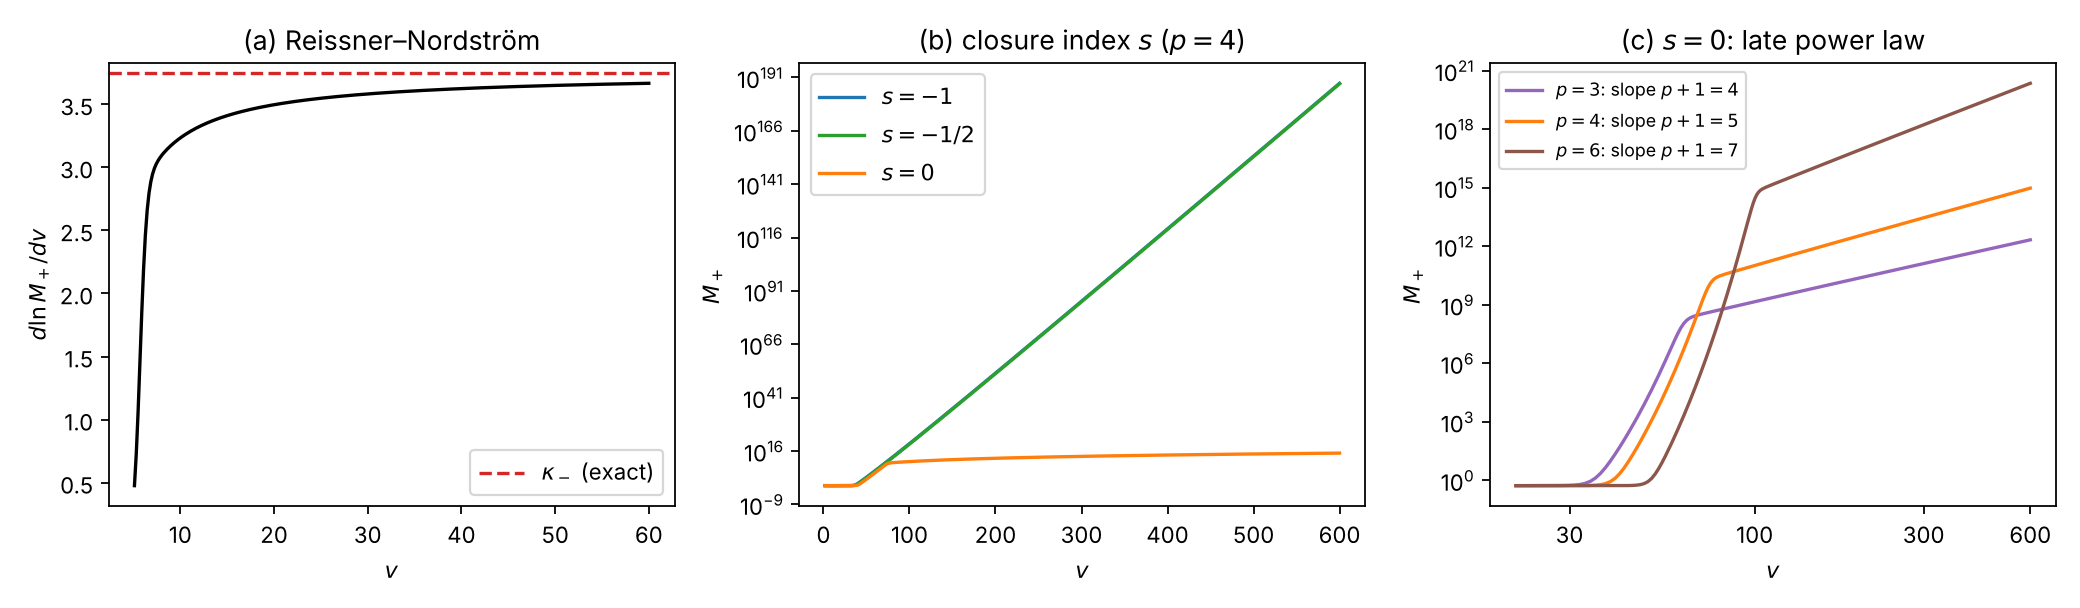
\includegraphics[width=\linewidth]{fig_ori_classes.png}
\caption{(a) Growth rate of $M_+$ for Reissner--Nordstr\"om approaches $\kappa_-$ (dashed). (b) $M_+(v)$ for closure indices $s=-1,-1/2,0$ ($p=4$); the curves for $s=-1$ and $s=-1/2$ coincide. (c) $s=0$ for three tail exponents: after the exponential phase the growth is a power law of slope $p+1$.}
\label{fig:classes}
\end{figure}

\section{Dependence on the closure}
\label{sec:classes}

Equation \eqref{eq:Mode} has a simple structure. The first term is a drag proportional to $G(M,R)$, with $\dot R<0$; the second is a linear drive with rate $\kappa_-$. At large $M$ the late behavior is therefore fixed by how $G$ grows with $M$, which is a property of the closure, not of the tail. Write $G\simeq gM^n$ at large $M$.

\paragraph{Regime I: no fold, $G$ linear ($-1\le s<0$).} For $-1<s<0$, $a(m)\propto m^{1+s}$ grows more slowly than $m$ but eventually exceeds $r^3$, so $M\to r^3(m/m_0)^{-s}/(2\ell_0^2)$ and $(m/m_0)^s\to r^3/(2\ell_0^2M)$; inserting in \eqref{eq:Gfamily} gives $G\to3M/R$ independently of $s$. For $s=-1$, $a$ is constant, $M$ is linear in $m$ and $G=(3M/R)\,a/(R^3+a)$. In both cases $G$ is linear in $M$ ($n=1$); we have not studied $s<-1$, where $a(m)$ decreases and $G\propto M^{2+s}$ is no longer linear; numerically $G/(3M/R)$ differs from $1$ by less than $10^{-13}$ (computed $3.2\times10^{-14}$, double-precision level; the exact deviation is $\sim R^3/a(m)$) at $M=10^{50}$ for $s=-1/2$. Then \eqref{eq:Mode} is linear at large $M$, $\dd\ln M_+/\dd v=\kappa_-+3\dot R/R-(p+1)/v+\dots$, and the $\dot R$ term is integrable, so $M_+$ grows exponentially without bound as $v^{-(p+1)}e^{\kappa_-v}$ as in the Reissner--Nordstr\"om case. Numerically the curves for $s=-1$ (where $M$ is linear in $m$) and $s=-1/2$ coincide to the plotted accuracy and their growth rates differ from $\kappa_-$ by $5.0/v$. The unbounded growth is non-uniform in $s$: reaching $M\gg R^3/2\ell^2$ requires $m_+\sim M^{1/|s|}$ (for $s=-0.01$, $M=6\times10^{5}$ at $v=60$ needs $m_+\sim10^{600}$), so this regime evaluates the closure at extreme parameters, and the limits $s\to0^\mp$ do not commute with the $s=0$ behavior.

\paragraph{Regime II: the M\"obius closure ($s=0$), followed through $m=\infty$.} For $a=2\ell^2m$, $M=mr^3/(r^3+2\ell^2m)$ is a fractional-linear function of $m$ with $\partial_mM=r^6/(r^3+2\ell^2m)^2>0$: it is monotone on the whole projective line, passes through $m=\infty$ at the finite value $M=r^3/2\ell^2$ and diverges at the pole $m=-r^3/2\ell^2$. Inverting, $m=Mr^3/(r^3-2\ell^2M)$ and $G=6\ell^2M^2/r^4$ ($n=2$). Hence the balance \eqref{eq:Msat}: exponential growth until $M_+\sim M_{\rm sat}$, then $M_+\propto v^{p+1}$. The passage through $m=\infty$ is regular (there $M=r^3/2\ell^2$ and the interior is exactly de~Sitter); the closure assumption is the continuation to negative $m$. The mass parameter does \emph{not} stay bounded along the way: it increases through $+\infty$ at the advanced time at which $M_+=R^3/2\ell^2$ ($v\approx36.6$ for $D_0=10^{-8}$, $p=4$, $\ell_0=1$, $m_0=m_\infty=5$, from a run in the regular variable $R^3/M_+$; \texttt{code/extra\_runs.py}) and re-emerges at large negative values, then tends to $-R^3/(2\ell^2)$. At that limit $a(m_+)=-R^3$, so $r^3+a$ vanishes at $r=R$: the geometry on the inner side of the shell is singular at the shell, which is what the divergence of $M_+$ means in this closure. This is the description of \citet{Bonanno2021} (the limit $m_+\to-r_-^3/2\ell^2$, their Eq.~(25), and polynomial growth of $M_+$ at $r_-$, their Eq.~(27)) and, in the other variable, of \citet{CarballoRubio2021}, who find that the integration for $m_+$ breaks down at a finite $v$ where $m_+$ diverges, continue it with $m_+<0$ approaching $-r_-^3/2\ell^2$, and call this an artifact of the parametrization; we identify that discontinuity and sign change with the passage through $m=\infty$ in our variable. We obtain the same limit and a power law with the exponent $p+1$ of \citet{CarballoRubio2021}; \citet{Bonanno2021} give $v^{p}$ for the same tail parametrization $m_-=m_0-\beta v^{-p}$, one power lower, a difference whose origin we have not traced. The contribution of this section is the identification of what separates this regime from the next.

\paragraph{Regime III: closure with a fold ($s>0$).} For $s>0$, $\partial_mM\propto r^3-s\,a(m)$ changes sign at a finite $m_*$, so $M(m,r)$ has a maximum $M_{\max}(r)$. On the branch with $\partial_mM<0$ at $m_\infty$ (this requires $s>R^3/a(m_\infty)\approx0.12$ for the parameters used; for $s=10^{-3},10^{-2},10^{-1}$ the fold is reached at finite $m_*=588,\,58,\,5.8$ with $m_+$ increasing), $M_+$ is driven up by the exponential term until it reaches $M_{\max}$, at which $\dd m_+/\dd v=S f_+/\partial_mM_+$ diverges: the model cannot continue because there is no value of $m_+$ with the required mass. As $s\to0^+$ the fold value approaches $R^3/2\ell^2$ (as $s\ln(1/s)$: $M_{\max}/(R^3/2\ell^2)=0.994,\,0.966,\,0.895$): runs at $s=10^{-3},10^{-2},10^{-1}$ stop at $v^*=36.55,36.17,32.41$ with $M_+=0.588,0.571,0.529$ against $R^3/2\ell^2=0.591$. The fixed-$\ell$ regime therefore differs from $s>0$ only in that its fold has been pushed to $m=\infty$, and the model is continued through it by the analytic form of the M\"obius map; that continuation is a closure assumption, not a consequence of the junction relation. For $s=1$, $M_{\max}=\sqrt{m_0R^3/(8\ell_0^2)}$ and for $s=2$, $M_{\max}=\tfrac23\bigl(m_0^2R^3/4\ell_0^2\bigr)^{1/3}$ (from $\partial_mM=0$); the numerical runs end at $0.859696$ and $1.298590$, the analytic values $0.859696$ and $1.298590$. Table~\ref{tab:fold} gives the finite advanced time $v^*$ at which this happens, which depends logarithmically on the seed ($v^*$ increases by $10.8$ and $10.2$ between successive seeds, each a factor $10^3$ or $6.9$ $e$-folds, i.e.\ $\approx1.5$ per $e$-fold of $D_0$, somewhat above $1/\kappa_-=1.26$ because the early growth rate is below $\kappa_-$ by $(p+1)/v$), while the value of $M_+$ reached is independent of the seed. For $s=2$ the pole of $M(m,r)$ at negative $m$ is not reached, because the fold intervenes first on the way up. This is not mass inflation: $M_+$ stays finite, bounded by the closure; it is a breakdown of the closure itself, which is a statement that the one-function description $M(m,r)$ cannot represent the interior of such a geometry once the shell energy has grown to order $R$, and a new closure (or a theory with the dynamical variable that $m$ stands for) is required.

\begin{table}[t]
\centering\small
\begin{tabular}{lcccc}
\toprule
$s$ & $D_0$ & $v^*$ & $M_+(v^*)$ & $M_{\max}$ (analytic)\\
\midrule
1 & $10^{-6}$ & 28.84 & 0.859696 & 0.859696\\
1 & $10^{-9}$ & 39.63 & 0.859696 & \\
1 & $10^{-12}$ & 49.8 & 0.859696 & \\
2 & $10^{-6}$ & 29.04 & 1.298590 & 1.298590\\
2 & $10^{-9}$ & 39.81 & 1.298590 & \\
2 & $10^{-12}$ & 50.0 & 1.298590 & \\
\bottomrule
\end{tabular}
\caption{Regime III: advanced time at which $M_+$ reaches the fold of the closure ($\ell_0=1$, $m_0=m_\infty=5$, $p=4$). The fold value does not depend on the seed $D_0$. The $D_0=10^{-12}$ rows are of the order of the integrator tolerance and are quoted to three digits.}
\label{tab:fold}
\end{table}

\paragraph{What the comparison says.} In the family $a\propto m^{1+s}$ the late behavior is exponential for $-1\le s<0$, a power law for $s=0$ only if the shell is continued through $m=\infty$, and a closure failure for $s>0$. The three regimes are a property of this family; we do not claim they classify all closures. The fixed-core-density metric of this series, $s=0$, sits at the boundary between regimes I and III, and its power-law behavior is the least robust of the three in the sense that any small $s>0$ stops the model at a value of $M_+$ that approaches the one where $s=0$ passes through. Paper~B's result is that the field equations do not determine $a(m)$, so the regimes are consequences of different assumptions, not different physics. The extremal tuning $q_a=16M^3/(27\ell^2)$ of \citet{EichhornFernandes2025} gives a single degenerate horizon ($r_-=r_+=4M/3$, so $\kappa_-=\kappa_+=0$), which is not the inner-extremal case ($\kappa_-=0$ with distinct horizons) treated by \citet{CarballoRubio2022b}; those authors' result does not apply to it, and the authors of the bi-Proca construction themselves flag a possible Aretakis-type instability of extremal horizons. We did not run that case.

\section{The evaporation clock}
\label{sec:evap}

The $e$-folding time of the instability is $1/\kappa_-\to\ell$; the time available is the lifetime of the hole. Paper~A \citep{PaperA} gives the evaporation law $\dd M/\dd u=-P(M)$ with $P=A\kappa_+^4/(960\pi^2)$ (normalized to the Hawking law \citep{Hawking1975,Page1976} $\hbar c^6/15360\pi G^2M^2$ for $M\gg\ell$; Planck units here), which behaves as $P\propto\varepsilon^2$ near $M^*$, so that $\varepsilon\propto1/u$. The total number of inner-horizon $e$-folds between masses $M_i$ and $M_f$ is
\begin{equation}
\Lambda=\int_{M_f}^{M_i}\frac{\kappa_-(M)}{P(M)}\,\dd M,\qquad u=\int_{M_f}^{M_i}\frac{\dd M}{P(M)}.
\label{eq:Lambda}
\end{equation}
For $M\gg\ell$, $\kappa_-=1/\ell$ and $P=1/(15360\pi M^2)$, so $\Lambda=5120\pi M_i^3/\ell\,$ in Planck units with $\ell=\ell_{\rm P}$; for a $10\,\Msun$ hole, $M_i/\ell\approx9.1\times10^{38}$ and $\Lambda\approx1.2\times10^{121}$. Table~\ref{tab:evap} shows the approach to this limit and the divergence as the final mass approaches $M^*$. Using the near-$M^*$ laws $\kappa_-=(\sqrt2/3)\sqrt\varepsilon/\ell$ and $\varepsilon=1/(\alpha\,u)$, $\alpha=1.513\times10^{-4}$ (\texttt{code/evap\_alpha.py}; not the core parameter $a(m)$ of \eqref{eq:closure}), with $\varepsilon_f=(M_f-M^*)/M^*$ the value at the final mass, one has
\begin{equation}
\Lambda\simeq\frac{2\sqrt2}{3\alpha}\,\varepsilon_f^{-1/2}\approx6.23\times10^{3}\,\varepsilon_f^{-1/2},
\end{equation}
confirmed numerically for $M_i=2\ell$ ($\Lambda\sqrt{\varepsilon_f}=8289,\;6494,\;6265$ for $\varepsilon_f=10^{-4},10^{-6},10^{-8}$, decreasing toward $6233$; the remainder $\Lambda-6233\,\varepsilon_f^{-1/2}$ is $2.1,\,2.6,\,3.2\times10^{5}$, slowly growing as $\varepsilon_f$ falls, which we have not analyzed). For $M_i\gg\ell$ the divergent term is a small fraction of $\Lambda$ (below $5\%$ for $M_i=20\ell$ even at $\varepsilon_f=10^{-6}$, Table~\ref{tab:evap}). The exponent therefore grows without bound, as $\sqrt u$, along the approach to $M^*$, which is itself never reached at finite $u$ (Paper~A). At fixed $M_i/\ell$ the near-$M^*$ constants scale as $(\ell/\ell_{\rm P})^2$; at fixed $M_i=10\,\Msun$, $\Lambda\propto1/\ell$.

\begin{table}[t]
\centering\small
\begin{tabular}{rrrrr}
\toprule
$M_i/\ell$ & $\varepsilon_f$ & $u$ [$t_{\rm P}$, $\ell=\ell_{\rm P}$] & $\Lambda$ & $\Lambda/(M_i^3/\ell)$\\
\midrule
20 & $10^{-1}$ & $1.31\times10^{8}$ & $1.21\times10^{8}$ & $1.51\times10^{4}$\\
20 & $10^{-4}$ & $2.01\times10^{8}$ & $1.22\times10^{8}$ & $1.52\times10^{4}$\\
20 & $10^{-6}$ & $6.78\times10^{9}$ & $1.27\times10^{8}$ & $1.59\times10^{4}$\\
$10^{3}$ & any & $1.61\times10^{13}$ & $1.61\times10^{13}$ & $1.606\times10^{4}$\\
$\to\infty$ & & & & $5120\pi\approx1.608\times10^{4}$\\
\bottomrule
\end{tabular}
\caption{Integrated inner-horizon exponent \eqref{eq:Lambda} over the evaporation from $M_i$ to $M^*(1+\varepsilon_f)$. For $M_i\gg\ell$ the exponent is $\approx M_i^3/\ell$ with coefficient $5120\pi$ and the final-mass dependence is lost because most of the exponent is accumulated at large mass.}
\label{tab:evap}
\end{table}

The interpretation needs care. $P$ is the geometric-optics law of Paper~A, without graybody factors, which overestimates the emission as $T\to0$ near $M^*$, so $u$ and $\Lambda$ near $M^*$ are order-of-magnitude and $10^{121}$ is to be read to one digit. $\Lambda$ is the exponent of the eternal-geometry growth rate integrated over the evaporation, not a prediction of the actual amplification, because the inner horizon of an evaporating hole is not the static one, the semiclassical stress at the Hayward inner horizon is not included (not computed here; \citet{Bonanno2023} report, at abstract level, that the Hawking flux can weaken or remove mass inflation in Hayward-type geometries), and the exponent is only meaningful while the thin-shell description holds. What it does say is that the instability, if present, has $\sim10^{121}$ $e$-folds to act, so that no tuning of the seed amplitude of a physically reasonable size can delay the onset beyond $\ln(1/D_0)\ell$, which is at most a few hundred $\ell$ even for $D_0=e^{-300}$. For comparison, \citet{FrolovZelnikov2026} find that for a single shell collision the amplification becomes large only within $x\sim\mu_C\mu_D\ell(\ell/r_g)^{2n(D-3)}$ of the inner horizon ($n=1$ for Hayward, $D=4$); in the continuous model the outgoing shell approaches the inner horizon exponentially, so that the condition is met, in this model, after a time of order $2\ln(r_g/\ell)/\kappa_-\approx180\,\ell$ for a $10\,\Msun$ hole at $\ell=\ell_{\rm P}$ (their Eq.~(4.20), taking $n=1$, which they find for the Hayward model, and $\mu_C\mu_D\sim1$ and an initial shell separation of order $\ell$ as our assumptions; with separation $r_g$ it is $\approx270\,\ell$). We note this as an observation about the two models and do not claim that it resolves the difference in their conclusions.

\section{A nonlinear test: Einstein--NED--scalar double-null evolution}
\label{sec:nonlinear}

The Ori model is a test-shell calculation: the shell does not react on the geometry through which it moves, so it cannot say whether the \emph{radius} of the inner horizon survives, and it contains no amplitude. The check we need is a nonlinear evolution with both ingoing and outgoing flux in a theory whose field equations fix the closure. \citet{ShaoEtAl2025} evolve a massless scalar field coupled to Einstein gravity and to a nonlinear-electrodynamics (NED) magnetic monopole that supplies the Hayward profile, with the back-reaction of the scalar included. We adopt a system of the same type: a NED monopole of fixed charge plus a massless scalar. We build our own code for it, with our own parameters and initial data, and have not compared the equations term by term with theirs, so the treatment of the NED sector (our additive closure) may differ. Everything below is a statement about this code, and the radius we measure (the area radius of the Cauchy horizon, $r_\infty$ below) is not shown to coincide with their ``inner-horizon radius''.

\subsection{System, closure and scheme}
\label{sec:nlsetup}

With $ds^2=-W\,du\,dv+r^2d\Omega^2$, $W=e^{\sigma}$, and the NED monopole stress tensor ($T_{uu}=T_{vv}=0$, $\rho=\rho(r)$, $p_r=-\rho$, $p_t=-\rho-r\rho'/2$) written through $M_N(r)=m_Nr^3/(r^3+a_N)$, $\rho=M_N'/(4\pi r^2)$, and a minimally coupled massless scalar with $\mathcal L=-\tfrac12(\partial\phi)^2$, i.e.\ $T_{ab}=\partial_a\phi\partial_b\phi-\tfrac12g_{ab}(\partial\phi)^2$, the field equations are
\begin{align}
r_{uv}&=-\frac{r_ur_v}{r}-\frac{W}{4r}\bigl(1-2M_N'(r)\bigr), \label{eq:dn1}\\
\sigma_{uv}&=-\frac{2r_{uv}}{r}-8\pi\phi_u\phi_v+\frac{W\,M_N''(r)}{2r},\label{eq:dn2}\\
\phi_{uv}&=-\frac{r_u\phi_v+r_v\phi_u}{r},\label{eq:dn3}
\end{align}
with the Misner--Sharp mass and the constraints
\begin{equation}
M=\tfrac r2\bigl(1+4r_ur_v/W\bigr),\qquad r_{uu}-\sigma_ur_u+4\pi r\phi_u^2=0\quad(\text{and }u\leftrightarrow v).
\end{equation} We derived \eqref{eq:dn1}--\eqref{eq:dn3} by hand and check them in \texttt{code/eh\_init/check\_field\_equations.py}: fields with prescribed second derivatives (finite-difference Riemann tensor of the four-dimensional metric, scalar plus NED-monopole stress tensor) obey $G_{ab}-8\pi T_{ab}=0$ in all four components to $3\times10^{-6}$ when \eqref{eq:dn1}, \eqref{eq:dn2} and the constraints are imposed, and each component departs by $0.07$--$1.6$ when its own second derivative is changed by $0.1$; $\Box\phi=0$ is \eqref{eq:dn3} to $10^{-15}$. The static Hayward interior is reproduced by the $A=B=0$ validation below. The closure is \emph{additive}, $M=\mu+M_N(r)$, where $\mu$ is the part of the mass carried by the scalar: $G=(\partial_rM)_m=M_N'(r)$ is independent of $M$, as in the Reissner--Nordstr\"om case; Section~\ref{sec:uniq} shows why this is the only closure a separately conserved dark sector allows. It is not the mass-tracking closure of this series ($a\propto m$): $a_N$ and $m_N$ are fixed by the NED charge, and the static sector of the mass-tracking closure is realized in four-dimensional quasi-topological gravity \citep{BorissovaCarballoRubio2026,BuenoCanoHennigar2024}, whose dynamics differ from this system (Paper~F, \citealp{PaperF}). The test therefore tests the method, the Ori law and the threshold in a Lagrangian system; it does not test the $s=0$ metric of the series. We use $m_N=5$, $a_N=10$ (so $\ell^2=a_N/2m_N=1$), for which the static interior has $r_-=1.057475$, $r_+=9.897927$, $\kappa_-=0.795649$, $\kappa_+=0.048969$.

\paragraph{Scheme.} The evolved variables are $r,\sigma,r_u,r_v,\sigma_u,\sigma_v,\phi_u,\phi_v$ (first-order form), so that quantities that are exponentially small near the Cauchy horizon, such as $r_u$, $r_v$ and $W$, keep full relative precision. The scheme is a double-null diamond scheme of the type used for scalar-field collapse \citep{GundlachPricePullin1994}, extended by evolving the first derivatives as independent variables: $r,\sigma$ are advanced by the diamond identity and the first derivatives by trapezoidal integration along the characteristic edges, with three predictor-corrector sweeps. Initial data on $v=0$ and on $u=-6$: $\sigma$ is set to its static value on both rays, $r$ follows from the Raychaudhuri constraint, $\phi=B+A\,e^{-u^2}$ on $v=0$ and $\phi=B(1+v)^{-k}$ on $u=-6$, $B=A/10$, $k=3/2$ unless stated. Prescribing $\sigma$ fixes the advanced time $v$ on the initial rays to be the static advanced time of the background, which is also the time in which the Ori tail is written; this matters for the interpretation below. The other natural prescription, fixing $r(v)$ to its static value and letting $\sigma$ follow from the constraint, forces $\sigma_v\sim e^{\kappa_-v}v^{-5}$ along the tail, so that $W$ underflows; it is a different, badly behaved data set, not a different physics, and is not used.

\paragraph{Validation.} For $A=B=0$ the code reproduces the static interior with error $1.1\times10^{-3},\,2.8\times10^{-4},\,6.9\times10^{-5},\,1.7\times10^{-5}$ at $h=0.08,\dots,0.01$ (measured order $1.998$--$2.000$). With a pulse, the $L_2$-norm of the relative Raychaudhuri residual in the $u$ direction is $2.2\times10^{-3},\,5.4\times10^{-4},\,1.4\times10^{-4}$ for $v\le20$ and $5.3\times10^{-3},\,1.3\times10^{-3},\,3.3\times10^{-4}$ for $20<v\le60$ at $h=0.08,0.04,0.02$ (order $2.00$); in the $v$ direction it is $1.2\times10^{-3},\,2.9\times10^{-4},\,7.3\times10^{-5}$ for $v\le20$ (and $3.4\times10^{-4},\,8.4\times10^{-5},\,2.1\times10^{-5}$ for $20<v\le58$). Grids are $u\in[-6,u_1]$, $v\in[0,v_1]$ with $h_u=h_v=h$.


\paragraph{Ray equations.} Along a ray $U=$ const (or $u=$ const), with $'=d/dv$, $\rho\equiv-r_v$, $y\equiv-r_u/W$ and $S(r)\equiv(1-2M_N'(r))/(4r)$, Eq.~\eqref{eq:dn1} and the Raychaudhuri constraint give the closed system
\begin{equation}
r'=-\rho,\qquad \rho'=\sigma_v\rho+4\pi r\phi_v^2,\qquad (\ln y)'=\frac{\rho}{r}-\sigma_v+\frac{S(r)}{y},\qquad M=\frac r2\,(1+4y\rho),
\label{eq:ray}
\end{equation}
and the part of the mass carried by the scalar, $\mu=M-M_N(r)$, obeys
\begin{equation}
\mu_v=-8\pi r^2\,\frac{r_u}{W}\,\phi_v^2=8\pi r^2\,y\,\phi_v^2\equiv g .
\label{eq:muv}
\end{equation}
These follow from Eqs.~\eqref{eq:dn1}--\eqref{eq:dn3} by elementary algebra; Paper~G \citep{PaperG} integrates them along rays of the evolved solution and tests them against it, and Paper~F \citep{PaperF} derives their analogue for the quasi-topological theory, where $\mu$ is replaced by the generalized mass.

\subsection{Why the nonlinear test is additive: a uniqueness statement}
\label{sec:uniq}

Write $ds^2=-W\,du\,dv+r^2d\Omega^2$ and let the dark sector have $T^u{}_u=T^v{}_v=-\rho$ (that is, $T_{uu}=T_{vv}=0$ and $\rho=-p_r$, the form of a nonlinear-electrodynamics monopole) and tangential pressure $p_t$. A direct computation of $\nabla_aT^a{}_b$ gives
\begin{equation}
\nabla_aT^a{}_u=-\rho_u-\frac{2r_u}{r}(\rho+p_t),\qquad \nabla_aT^a{}_v=-\rho_v-\frac{2r_v}{r}(\rho+p_t),\label{eq:consT}
\end{equation}
which we also checked by finite differences against the brute-force covariant divergence for arbitrary smooth $r,\sigma,\rho,p_t$ (\texttt{conserv\_num.py}: agreement to $10^{-11}$ in both components, at one point with one set of test functions; the formula was also derived by hand from $\nabla_aT^a{}_b=(-g)^{-1/2}\partial_a(\sqrt{-g}\,T^a{}_b)-\tfrac12\partial_bg_{cd}T^{cd}$). Separate conservation of this sector is an assumption (only the total is conserved by the Bianchi identity). If it holds, both components vanish, so $\rho_ur_v=\rho_vr_u$, that is $d\rho\wedge dr=0$: where $dr\ne0$, $\rho=\rho(r)$ is locally a function of the area radius alone, and the static relation $p_t=-\rho-r\rho'/2$ follows. Its contribution to the Misner--Sharp mass is then $M_N(r)=\int4\pi r^2\rho\,dr$, and the total mass is $M=\mu+M_N(r)$ with $\mu$ the scalar's share, which obeys Eq.~\eqref{eq:muv}. This is the additive closure of Section~\ref{sec:nlsetup}. \emph{Statement:} the assumptions are (a) the dark sector is conserved on its own, (b) it has the monopole form $T_{uu}=T_{vv}=0$, $T^u{}_u=T^v{}_v=-\rho$, with tangential pressure $p_t$, (c) it does not couple directly to $\phi$ (implied by (a)), (d) the conclusion is local, where $dr\neq0$, and (e) the relabeling $m\mapsto F(m)$ is monotonic. Under these assumptions a separately conserved dark sector produces only closures with $\partial_m\partial_rM=0$, i.e.\ $M=F(m)+M_N(r)$ (equivalently $M=m+M_N(r)$ after relabeling $m$), where $m(u,v)$ is not a function of $r$ alone; the mass-tracking closure $a\propto m$ of the series (for which the $r$-dependence of $M$ changes with $m$), and every other member of the family \eqref{eq:family} with $\partial_m\partial_rM\neq0$, cannot. They need $\rho=\rho(r,m(u,v))$ with $\nabla_aT^a{}_b\neq0$, i.e.\ an energy and momentum exchange with the scalar that is not derived from an action here. The statement does not cover dark sectors with $T_{uu},T_{vv}\ne0$ (scalar-like), nor non-spherical ones. It explains why the nonlinear test is restricted to $M=\mu+M_N(r)$ and sharpens the open item of Paper~B \citep{PaperB}: the mass-tracking metric needs a coupled dark sector, and that coupling is the missing theory.

\subsection{Below threshold: mass inflation at the Ori law, with a finite radius}
\label{sec:below}

For weak data the Misner--Sharp mass on the Cauchy horizon grows exponentially while $r$ converges in $v$ to a finite $r_{CH}(u)$: $|r(v{=}100)-r(v{=}50)|/r\le2\times10^{-11}$ at $u=4$ and $u=40$ for $A=0.02$, and $\le4\times10^{-5}$ even at $A_*-A=10^{-10}$ (the approach there is a power law in $v$, not an exponential). We compare $d\ln|M|/dv$ with the Ori shell model run with the matching additive closure (a new closure \texttt{hn} in \texttt{ori\_model.py}; its tail $m_-(v)=-\delta v'^{-4}$, $v'=v+1$, corresponds to $\phi_v^2\propto(1+v)^{-5}$, and $\delta$ is varied over a factor $10$):
\begin{table}[h]
\centering\small
\begin{tabular}{p{0.60\textwidth}cc}
\toprule
& $d\ln|M|/dv$ at $v=79$ & at $v=98$\\
\midrule
double-null PDE, $A=5\times10^{-4}$ to $2\times10^{-2}$, $u\in\{-3,0,2,5\}$ & $0.73203$--$0.73212$ & $0.74444$\\
Ori shell model, additive closure, $\delta=10^{-3},10^{-2}$ ($v'=v+1$) & $0.73204$ & $0.74444$\\
$\kappa_--5/(v+1)$ (leading order) & $0.73315$ & $0.74514$\\
\bottomrule
\end{tabular}
\caption{Growth rate of $|M|$ on the Cauchy horizon, windows $\pm1$ in $v$. The $(A,B)$ pairs are $(0.02,0.002)$, $(0.01,0.01)$, $(0.005,0.001)$ and $(5\times10^{-4},10^{-4})$. Only the smallest amplitude ($5\times10^{-4}$) departs from $0.732038$ by more than $10^{-6}$ at $v=79$ (by $8\times10^{-5}$ at $u=-3$, $2\times10^{-5}$ at $u=2$, $6\times10^{-6}$ at $u=0$); at $v=98$ the spread of the PDE rates is $\le6\times10^{-7}$ for all runs. The difference from the leading-order law ($7.1/(v+1)^2$ and $6.9/(v+1)^2$) is the next term, which the shell model has as well. At $u=30,40$ and $A_*-A=10^{-10}$ the rates are $0.73198$ and $0.74441$, a small shift that we did not investigate.}
\label{tab:nlrate}
\end{table}
The two (Table~\ref{tab:nlrate}) agree to $7\times10^{-7}$ at $v=79$ (all runs but the smallest amplitude) and to $4\times10^{-7}$ at $v=98$ (all runs). The rate is the same at the $u$ we measure ($u=-3,0,2,5$) and, but for the smallest amplitude, does not depend on the amplitude in this gauge for $v\gtrsim75$; at earlier $v$ it does (at $v=59$ the rate is $0.7102$ for most runs but not for the weakest, where the exponential phase has not yet set in, and the onset moves with the amplitude ($1.92$ at $u=-3$ for $A=0.005$; irregular for $A=5\times10^{-4}$); at $u=-3$ it is grid dependent, $0.7334$ and $0.7388$ for $A=0.02$, $B=0.002$ on two grids), and at the single $u_\star\approx-1.88$ where $M$ changes sign the coefficient of the leading term vanishes. In this gauge the amplitude changes the coefficient, not the rate: $|M(u{=}2,v{=}100)|$ ranges from about $10^{11}$ to $5\times10^{18}$ over the amplitudes (and is negative at the smallest).

The tail sets the exponent. With $\phi\propto(1+v)^{-k}$ on the ingoing ray the Ori law $M\propto e^{\kappa_-v}v^{-(p+1)}$, $p=2k+1$, predicts $q\equiv(\kappa_--\text{rate})(v+1)\to2k+2$; the PDE gives, at $v=98$, $q=4.055,\,5.070,\,6.085,\,7.101$ for $k=1,\,3/2,\,2,\,5/2$ (and $4.080,\,5.102,\,6.125,\,7.150$ at $v=70$), the excess over $2k+2$ decreasing as $1/v$ and identical to that of the Ori ODE for $k=3/2$ ($5.070$).

\paragraph{What is and is not measured here.} With $\sigma$ prescribed on the initial rays and $\sigma_{uv}\to0$ at late $v$, the PDE has $\sigma_v\to-\kappa_-^{\rm static}$ at every $u$ and every amplitude (we measured $-0.795649$ at $u=-3,0,2,5$ for all five amplitude and grid combinations of \texttt{run\_rates.py}), so that $M\simeq2rr_ur_v/W$ grows as $e^{\kappa_-^{\rm static}v}$ times the power law of $r_ur_v$ \emph{by construction of the gauge}. The dynamical content of the table is therefore (i) the power law $r_ur_v\propto v^{-(2k+2)}$ with its $O(v^{-2})$ correction, (ii) the finiteness of $r_{CH}$, and (iii) the agreement of the full rate curve with the Ori ODE in the same time variable. The equality of the exponent with $\kappa_-^{\rm static}$ is not an independent measurement of the surface gravity: a shift of the effective $\kappa_-$ at $O(A^2)$ from the mass accumulated on the ingoing ray, which a time variable tied to the final geometry would show, is invisible in this gauge, and it is not tested in this subsection; Section~\Gehdatan{} of Paper~G tests it with data on the event horizon, where $v$ is the exterior time. The sign of $M$ is not uniform: for $A=0.02$, $B=0.002$ at $h=0.04$, $M<0$ for $u<-1.88$ and $M>0$ above at $v=100$; at the smallest amplitude the sign pattern is irregular and grid dependent. The sign change has a mechanism, and it is exact. With $y\equiv-r_u/W$ and $\rho\equiv-r_v>0$ the Misner--Sharp mass is $M=\tfrac r2+2ry\rho$ (Eq.~\eqref{eq:ray}), so $M-r/2$ has the sign of $-r_u$; Eq.~\eqref{eq:muv} (derived below) gives the same for the growing part, $\mu_v=-8\pi r^2(r_u/W)\phi_v^2$. The $u$-Raychaudhuri equation gives, moreover, $\partial_u(r_u/W)=-4\pi r\phi_u^2/W\le0$ at fixed $v$: $r_u/W$ is non-increasing in $u$, so $r_u$, and with it the sign of the inflating mass, changes sign at most once along a slice, from $r_u>0$, $M<0$ at small $u$ to $r_u<0$, $M>0$. The runs agree. For $A=0.02$, $B=0.002$, $h=0.04$ the sign changes of $M$ and of $r_u$ at $v=100$ occur at the same grid interval, $u=-1.88$ (\texttt{code/nonlinear/sign\_mech.py}, \texttt{sign\_mech.log}): $r_u>0$ and $M<0$ for $u<-1.88$, $r_u<0$ and $M>0$ for $u>-1.88$, and $r_u(v=100)=r_u(v=50)$ at every $u$ listed, so the sign is fixed early; the radius $r_{CH}(u)$ has its maximum at $u\approx-1.92$. \texttt{sign\_scan.py} (\texttt{sign\_scan.log}) repeats the run for seventeen combinations of amplitude ($5\times10^{-4}\le A\le0.0204$), tail amplitude ($10^{-4}\le B\le0.02$) and grid ($h=0.08,\dots,0.01$). In each of them, except the two coarsest runs at the smallest amplitude (below), $r_u$ and $M$ change sign exactly once and at the same $u$, and $\operatorname{sign}M=-\operatorname{sign}r_u$ at every point with $|M|>10r$ (fraction $1.0000$). The position $u_\star$ depends on the data: $-1.44,\,-1.68,\,-1.88,\,-1.92$ for $A=0.005,\,0.01,\,0.02,\,0.0204$ at $B=0.002$ and $h=0.04$; $-2.04,\,-1.88,\,-1.48,\,-1.0$ for $B=0.0005,\,0.002,\,0.01,\,0.02$ at $A=0.02$; with $h$ it moves by the grid spacing ($-1.84,\,-1.88,\,-1.94,\,-1.94$ for $h=0.08,\,0.04,\,0.02,\,0.01$). The irregular, grid-dependent sign pattern at the smallest amplitude ($A=5\times10^{-4}$, $B=10^{-4}$) is a violation of the monotonicity by truncation: $r_u/W$ increases along $u$ by $6\times10^{-2}$, $3\times10^{-2}$ and $8\times10^{-3}$ of its maximum modulus at $h=0.04,\,0.02,\,0.01$ (against $\le7\times10^{-5}$ in all other runs), and at $h=0.01$ there is a single sign change, at $u=-1.24$. This is the nonlinear counterpart of the orientation $D_0$ of the Ori model (Section~\ref{sec:model}), which there is a choice and here is a consequence of the data. What fixes $u_\star$ in terms of the data on the initial rays we have not derived, but its character is exact. The ray equation (Eq.~\eqref{eq:ray}) is linear in $y$, $y'=ay+S$, with $a=\rho/r-\sigma_v\to\kappa_->0$ and $S=(1-2M_N')/(4r)<0$ at $r_-$, both fixed along the ray by the $v$-constraints. Hence $y(v)-y_{\rm sep}(v)=\Phi(v)\,[y(v_0)-y_{\rm sep}(v_0)]$ with $\Phi=\exp\int_{v_0}^va\,dv$ and the bounded solution $y_{\rm sep}(v_0)=-\int_{v_0}^\infty S\,\Phi^{-1}dv$, the stable manifold of the unstable fixed point $y\simeq\tfrac12$. A ray with $y(v_0)>y_{\rm sep}$ has $y,M\to+\infty$ and one with $y(v_0)<y_{\rm sep}$ has $y,M\to-\infty$: $u_\star$ is the ray on which the mass does not inflate, and the sign is decided when the ray enters the exponential regime, not by the data at the last $v$. Numerically (\texttt{sign\_ustar.py}, \texttt{sign\_separatrix.py} and their logs; three of the runs above) $u_\star$ does not move for $v\ge30$ ($-1.8790$, $-1.1565$, $-1.5430$ for $(A,B)=(0.02,0.002),\,(0.01,0.01),\,(0.005,0.001)$ at $h=0.04$, from $v=30$ to $100$, to the printed digits), and the zero of $y(v_0,u)-y_{\rm sep}(v_0,u)$, with $y_{\rm sep}$ computed from the evolved ray fields, lies at the same $u$ for each of $v_0=30,40,50$ ($y_{\rm sep}=0.4990$, $0.4715$, $0.4998$). Since $y(v_0,u)$ is very steep there ($|\partial_uy|>10^4$) this says that the zero of $r_u$ on the slice at $v_0$ is the separatrix to $10^{-5}$ in $u$, i.e.\ that the sign is decided by $v\approx30$ and persists, as the linear equation demands; it does not give $u_\star$ in terms of $A$ and $B$. For the data regular on the event horizon $y=\tfrac12+\int4\pi r\phi_s^2/W\,ds>\tfrac12$ on the whole slice (Section~\Grayn{} of Paper~G), and the mass is positive and inflating on every ray computed ($U\simeq0.3$--$1.2$): no sign change occurs there. The relation fixes the sign of the growing part only where the mass parameter at the start of the inflation is negligible and $\phi_v$ has no node.

\subsection{Threshold and critical scaling}

For a fixed data family ($u_1=40$, $v_1=50$) there is a critical amplitude $A_*$ above which $r$ reaches zero (we flag $r\le10^{-5}$ or non-finite fields) and below which $r_{CH}$ stays finite. $A$ is the amplitude of $\phi$ on the initial ray in these coordinates, so $A_*$ is not an invariant energy threshold, and ``weak'' means only $A<A_*$. $A_*$ is converged in the domain ($0.022204,\,0.021146,\,0.020468,\,0.0204297,\,0.02042799,\,0.02042799$ for $u_1=6,8,12,16,24,32$, $h=0.04$, criterion $r\le10^{-3}$; the sensitivity at small $u_1$ is the collapse occurring at the outer edge, which the domain then truncates), independent of $v_1$ (identical to eleven digits for $v_1=40,60,80,100$ at $u_1=8$), and second-order in the grid: $A_*=0.0204360,\,0.0204280,\,0.0204260$ at $h=0.08,0.04,0.02$, Richardson limit $0.0204253$. The flag offsets $A_*$ from the true critical value by $(r_{\rm flag}/41)^2$, which is $6\times10^{-14}$ for $r_{\rm flag}=10^{-5}$ and $6\times10^{-10}$ for $10^{-3}$. The radius $r_{CH}(u)$ falls with $u$ for $u\gtrsim-2$ and saturates (Figure~\ref{fig:nl}d); we take $r_\infty=r_{CH}(u{=}40)$, which agrees with $r_{CH}(u{=}50)$ to $4\times10^{-5}$ even at $A_*-A=10^{-10}$ (at that distance $r_{CH}(30)$ is still $12\%$ larger than $r_{CH}(40)$; \texttt{code/nonlinear/check\_saturation.py}, written after the original work, gives $4.4\times10^{-5}$ and $11.8\%$). The dependence of $r_\infty$ on $A_*-A$ is consistent with a square root over the last one to three decades (the data span $10^{-10}$ to $10^{-3}$, but the local exponent leaves $1/2$ beyond $\sim10^{-6}$: $0.43$ at $2.5\times10^{-5}$ and $0.24$ at $10^{-3}$),
\begin{equation}
r_\infty\simeq41\,(A_*-A)^{\gamma},\qquad \gamma=0.4997\pm0.002,
\label{eq:gamma}
\end{equation}
where $0.4997$ is the fit over $[10^{-10},10^{-9}]$ and the uncertainty is the spread over fit windows (not a statistical error), the prefactor is $40.8,\,41.2,\,41.3$ at $h=0.08,0.04,0.02$ and the local exponent $d\ln r_\infty/d\ln(A_*-A)$ (central difference) is $0.4995$--$0.4998$ for $A_*-A\le1.6\times10^{-9}$ on all three grids ($0.4999$ at $10^{-10}$ after correcting for the flag offset), $0.4960$ at $10^{-7}$ and $0.43$ at $2.5\times10^{-5}$ (Figure~\ref{fig:nl}b,c). Fits over $[10^{-10},10^{-9}]$, $[10^{-10},10^{-7}]$ and $[10^{-10},10^{-6}]$ give $0.4997$, $0.499$ and $0.498$ (\texttt{code/nonlinear/fit\_gamma.py}, \texttt{fit\_gamma.log}); the exponent drifts away from $1/2$ beyond $A_*-A\sim10^{-6}$ and we do not claim a power law there. For the other data families we tried the local exponent is the same: a pulse of width $2$ ($A_*=0.026673$; $0.499$--$0.500$ over $A_*-A\in[10^{-10},10^{-7}]\times A_*/0.02$), $B=A/2$ ($A_*=0.018039$; $0.499$--$0.500$) and a steeper tail $k=2$ ($A_*=0.020385$; $0.497$--$0.500$), all at $h=0.04$; $A_*$ and the prefactor are data dependent, and the three families share the Gaussian-plus-power-tail form and the parameters $(m_N,a_N)$. \citet{ShaoEtAl2025} report $\gamma\approx0.5$ (fits $0.4995$--$0.5001$ for the amplitude, the width and the position of a Gaussian initial profile); our value is consistent with it, and this is a comparison of exponents, not a reproduction. A square root is what one expects if $r_\infty^2$ is a smooth function of $A$ with a simple zero at $A_*$; we have not derived that for the present system, so the exponent is not by itself a diagnostic of a particular mechanism. Above threshold the locus $r=0.05$ lies at $v_s(u)$ decreasing with $u$ (spacelike) for moderate $u$ and tends to a constant $v$ (a null ray) at large $u$, for $A/A_*=1.0005$, $1.01$, $1.05$, $1.3$; we did not resolve the endpoint $r\to0$, nor examine what happens beyond it.

\begin{figure}[t]
\centering
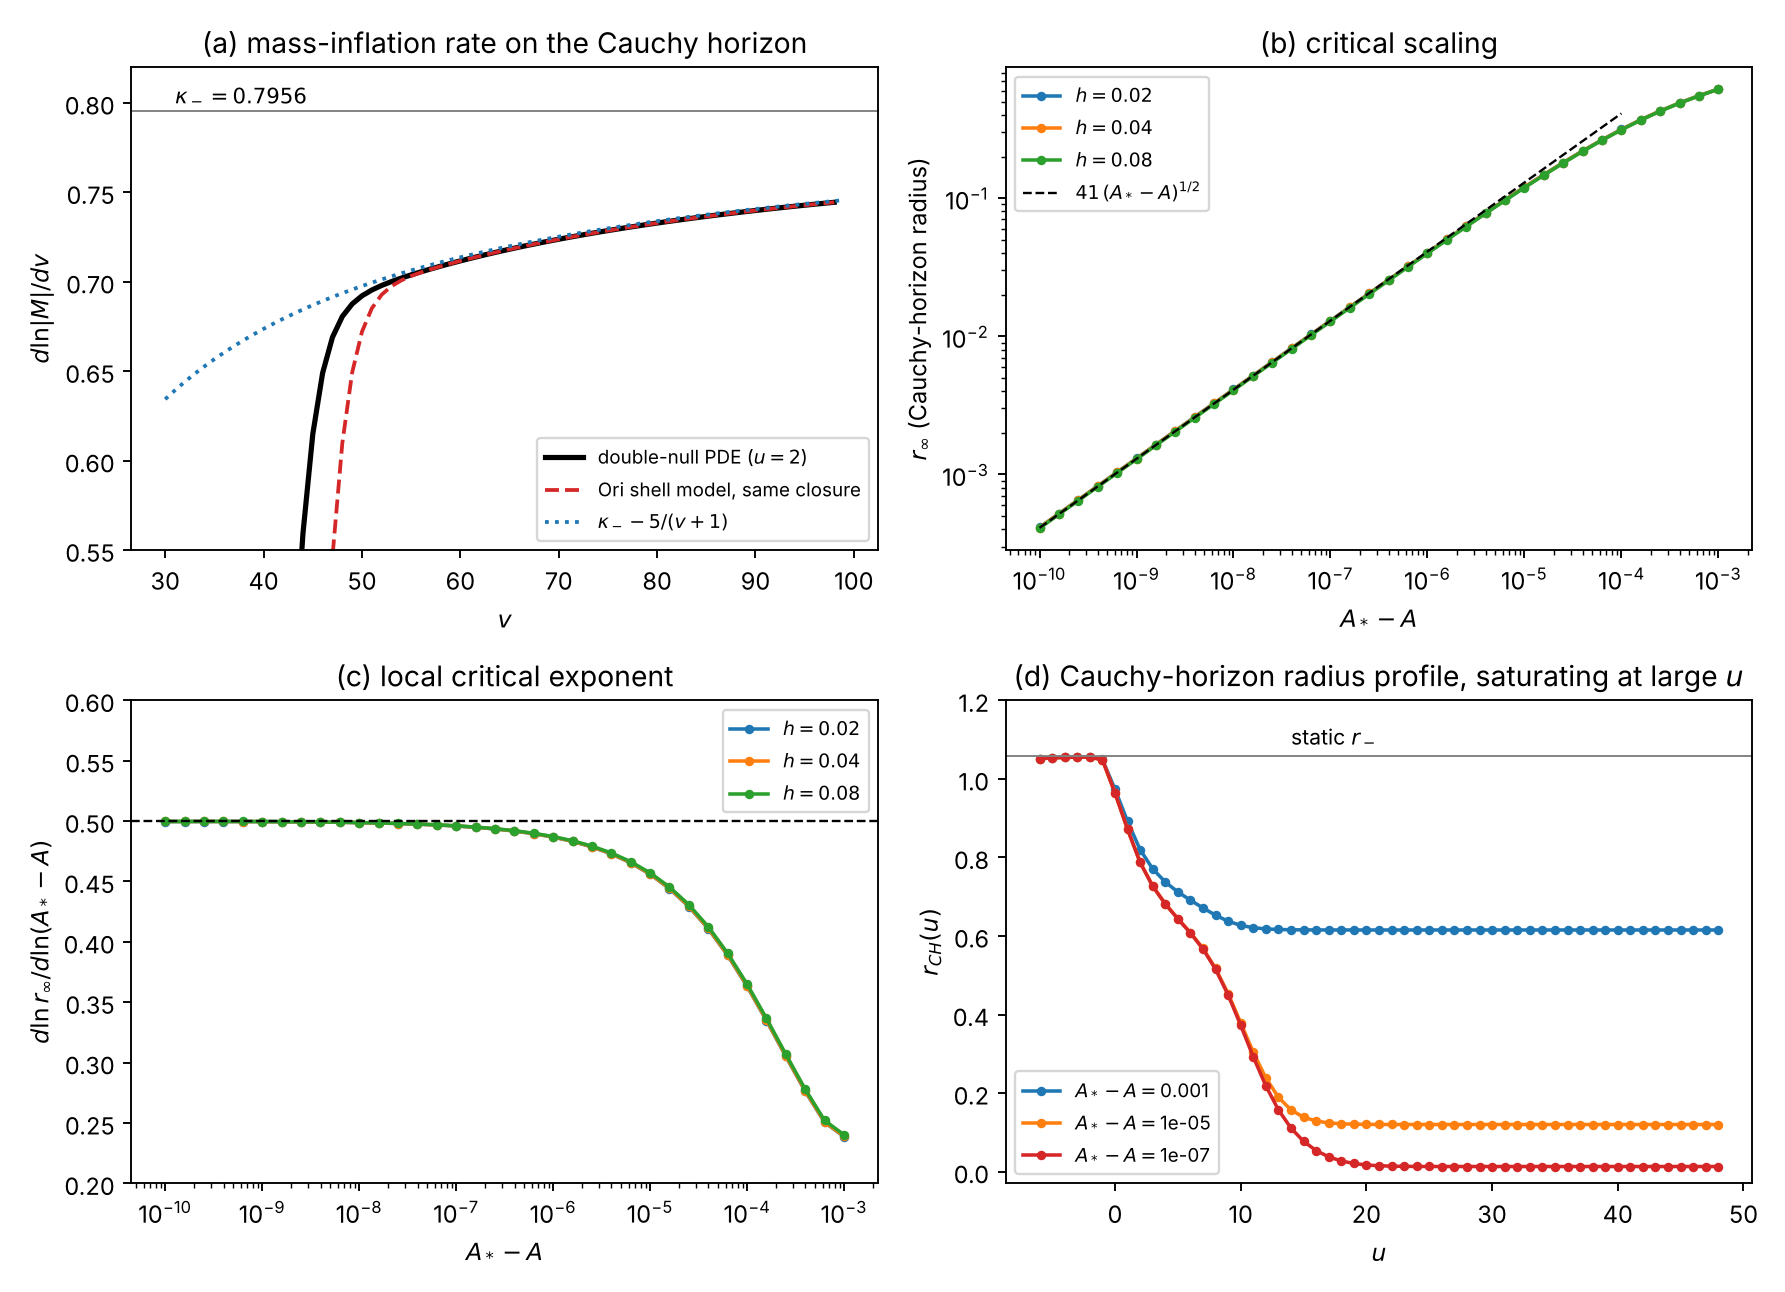
\includegraphics[width=0.96\textwidth]{fig_nonlinear.png}
\caption{Nonlinear Einstein--NED--scalar evolution (additive Hayward closure, $m_N=5$, $a_N=10$). (a) Growth rate of $|M|$ on the Cauchy horizon: PDE ($A=0.02$, $B=0.002$, $u=2$, $h=0.04$), Ori shell model with the same closure, and the leading-order law; the PDE and the shell model coincide after the exponential phase has set in. (b) Cauchy-horizon radius $r_\infty$ against the distance below threshold; three grids overlap. (c) Local critical exponent. (d) $r_{CH}(u)$ for three distances to threshold.}
\label{fig:nl}
\end{figure}

\subsection{Curvature on the Cauchy horizon}
\label{sec:curv}

The Misner--Sharp mass is not an invariant that can be read as curvature on its own, so we evaluated the Kretschmann scalar from the stored fields. In spherical symmetry $\mathcal K=R_2^2+8H_{AB}H^{AB}/r^2+4(2M/r)^2/r^4$, with $R_2=4e^{-\sigma}\sigma_{uv}$ the curvature of the 2D orbit space, $H_{AB}=\nabla_A\nabla_Br$, $H_{uu}=-4\pi r\phi_u^2$ and $H_{vv}=-4\pi r\phi_v^2$ (from the constraints), $H_{uv}=r_{uv}$ and $H_{AB}H^{AB}=(8/W^2)(H_{uu}H_{vv}+H_{uv}^2)$; the multiplicities were derived from the Riemann components and are checked in \texttt{check\_field\_equations.py} against the full contraction $R_{abcd}R^{abcd}$ of a finite-difference Riemann tensor of the four-dimensional metric, for generic fields: relative differences $6.5\times10^{-6}$ and $4.5\times10^{-6}$ for two sets of fields. In the code the static ($\phi=0$) value is reproduced to $2.0\times10^{-4}$ at $h=0.04$ (second order).

For $A=0.02$, $B=0.002$ at $u=2$, $\mathcal K$ rises from $25.7$ at $v=20$ ($25.67$ at $h=0.04$; static value $12.3$; \texttt{run\_curvature.py}, whose $v=20$ row and static value were added to its output after the original run) to $2.5\times10^{50}$ at $v=100$ ($0.5\%$ change between $h=0.04$ and $h=0.02$). From $v\approx30$ it is dominated by the first two terms, which are equal to four digits from $v\approx40$, and
\begin{equation}
\mathcal K=2048\pi^2\left(\frac{\phi_u\phi_v}{W}\right)^{2}=128\pi^2\bigl[(\nabla\phi)^2\bigr]^2 .
\label{eq:Kscalar}
\end{equation}
The constant is analytic: once $r_ur_v/W$ and $M$ are negligible, \eqref{eq:dn2} gives $\sigma_{uv}/W\to-8\pi\phi_u\phi_v/W\equiv-8\pi Y$ and $R_2^2=16(\sigma_{uv}/W)^2=1024\pi^2Y^2$, and $8H_{AB}H^{AB}/r^2=64H_{uu}H_{vv}/(r^2W^2)=1024\pi^2Y^2$, whose sum is \eqref{eq:Kscalar}; numerically the ratio is $1$ to $1.5\times10^{-5}$ at $v=98$ for $u=-3,0,2,5$, for amplitudes $0.005$, $0.02$ and $0.0204\approx A_*$, and for tails $k=1,\,3/2,\,2$. Here $\phi_u$ stays finite and non-zero on the horizon ($-7.4\times10^{-3}$ at $u=2$), $\phi_v\propto v^{-k-1}$ and $W\propto e^{-\kappa_-v}$, so that $d\ln \mathcal K/dv=2\kappa_--(2k+2)/(v+1)$: $1.54079$ at $v=98$ for $k=3/2$, measured $1.54079$ (and $1.55089$, $1.53069$ for $k=1,2$, both measured to the printed digits). The scaling of $\mathcal K$ is a property of the gauge and of the imposed tail: $W\propto e^{-\kappa_-v}$ and $\phi_v\propto v^{-k-1}$ are inputs, and only the finiteness of $\phi_u$ on the horizon is measured. The mass-function term of $\mathcal K$ is smaller by thirteen orders of magnitude at $v=100$ (measured there; we have not derived its $v$-dependence); $M$ also enters through $r_{uv}$, a correction of relative size $\sim10^{-6}$ to \eqref{eq:Kscalar}. With $\mathcal K=C^2+2R_{ab}R^{ab}-R^2/3$ and $R_{ab}\simeq8\pi\partial_a\phi\partial_b\phi$ the Weyl invariant is $C^2\simeq \mathcal K/6$ (an estimate from these relations; we did not compute $C^2$ separately), so the divergence is not purely a Ricci effect. In summary the curvature grows without bound along the Cauchy horizon up to $v=100$ at finite radius ($r=0.80$ at $u=2$), through the combination of the ingoing tail and the finite outgoing flux, and not through $M^2$.

This suggests that the solution is not $C^2$-extendible through the horizon. The argument is numerical, extrapolated from $v=100$ (it assumes that the scalings continue to $v=\infty$), and holds for this data class and this closure only. The ray $u=\text{const}$ is a null geodesic with affine parameter $d\lambda=W\,dv$ (because $\Gamma^v_{vv}=\sigma_v$), $W\,e^{\kappa_-v}=91.04$ for $v=40$--$100$ and $\sigma_v=-0.795649$ there, so the affine length of the part of the ray beyond $v=100$ is $W(100)/\kappa_-\approx3\times10^{-33}$ against $7.33$ up to $v=100$ ($u=2$). If $\mathcal K$ diverges along a geodesic of finite affine length, a $C^2$ extension is ruled out, since in it the geodesic would continue and $\mathcal K$ would stay continuous. This does not decide extendibility in the weaker senses (a continuous metric across the horizon, a weak null singularity in which integrated tidal distortions stay finite); we did not compute geodesic deviation, and the indicators at the end of this subsection are not that computation.

\paragraph{A lower bound that does not use the scalings.} Every term of $\mathcal K$ is non-negative: $R_2^2$ is a square, $H_{AB}H^{AB}=(8/W^2)(H_{uu}H_{vv}+H_{uv}^2)$ with $H_{uu}H_{vv}=16\pi^2r^2\phi_u^2\phi_v^2\ge0$, and the mass term is a square. Hence $\mathcal K\ge16M^2/r^6$. On the rays $U\simeq1$ of the event-horizon-regular runs, where $M$ and $r$ are known to $v=280$ (Section~\Grayn{} of Paper~G; $r\simeq1.04$--$1.06$, the Cauchy-horizon radius at finite $r$), this gives $\ln\mathcal K\ge337,\,360,\,323,\,343$ at $v=280$ for $(k,B)=(3/2,0.03),\,(1/2,0.03),\,(3/2,0.003),\,(1/2,0.003)$ (last column of Table~\Gtabproj{} of Paper~G), and the bound grows as $2\ln M$, i.e.\ at the rate $2\kappa_-$ up to powers of $v$. The divergence of $\mathcal K$ along the ray at finite $r$ therefore follows from the growth of $M$ alone, without the extrapolation of $W\propto e^{-\kappa_-v}$ and $\phi_v\propto v^{-k-1}$ used above; it is a statement about $v\le280$ in the nonlinear run (and about the kernel-driven extension beyond), for this data class and closure. For the data of the $(u,v)$ runs above the mass term is not the leading one at $v=100$ ($13$ orders below the other terms), so the bound is weaker than the asymptotics there but of the same exponential rate.

\paragraph{Weaker senses of extendibility: two indicators.} The theorems that bear on this question are for related systems: for the spherically symmetric Einstein--Maxwell--scalar-field system with Price-law tails on the event horizon the spacetime extends across the Cauchy horizon with a continuous metric, while the Hawking mass blows up identically along it, so that no differentiable extension exists \citep{Dafermos2005} (abstract-level reading); for the spherically symmetric Einstein--Maxwell--Klein--Gordon system (charged scalar field), under a decay assumption on the event horizon, the Cauchy horizon emanating from timelike infinity is $C^2$-inextendible \citep{VanDeMoortel2020} (abstract-level). The system here (nonlinear electrodynamics with the additive closure, a neutral scalar) is outside their hypotheses, so we do not quote their conclusions for it; we compute along the rays of the event-horizon-regular runs the two quantities that such statements rest on. \emph{(i) Continuity of the metric.} In the coordinate $V=-e^{-\kappa_-(\mu_f)v}$, which is regular at the Cauchy horizon, the metric component is $W_{sV}=W\,e^{\kappa_-v}/\kappa_-=e^{\Lambda}/\kappa_-$ with $\Lambda(v)=\sigma(v)+\kappa_-(\mu_f)v$ ($s$ is the ray label; the area radius is finite, Section~\Grayn{} of Paper~G). A finite positive limit exists if and only if $\Lambda$ converges, i.e.\ if and only if $\int^\infty(|\sigma_v|-\kappa_-(\mu_f))\,dv$ converges. \emph{(ii) Weakness of the singularity.} A worldline that crosses the Cauchy horizon transversally has $d\tau\propto|dV|\propto e^{-\kappa_-v}dv$. The mass term of the curvature is $\sim M/r^3$, and the matter terms of $\mathcal K$ (the dominant ones in Eq.~\eqref{eq:Kscalar}) are $\sim\phi_s\phi_v/W$ in the coordinate frame, so the tidal integrals along the worldline are
\begin{equation}
J(v)=\int^{v}\frac{M}{r^{3}}\,e^{-\kappa_-v'}dv',\qquad J_\phi(v)=\int^{v}\frac{|\phi_s\phi_v|}{W}\,e^{-\kappa_-v'}dv'=\int^{v}|\phi_s\phi_v|\,e^{-\Lambda(v')}dv',
\label{eq:tidal}
\end{equation}
and the distortion of an extended body is finite if both converge (a body crossing is stretched by $\iint\!R\,d\tau d\tau$; the normalization of $d\tau$ depends on the worldline, so the integrals are judged only for convergence; this is the sense in which the mass-inflation singularity is called weak \citep{Ori1991}; we use it as a criterion and do not re-derive it). We used the projected mass $M_{\rm cc}$ for $M$ and the extrapolated $\sigma$, $\sigma_v$, $\phi_s$, $\phi_v$ (\texttt{e15\_extend.py}, \texttt{results\_e15\_extend.txt}). Table~\ref{tab:ext} gives the results. For $k\ge3/2$, $\Lambda$ and $J$ have converged to $10^{-3}$ or better and $J_\phi$ to $10^{-2}$ by $v=280$: $\Lambda$ changes by $0.016$, $0.011$, $0.009$ between $v=100$ and $280$ ($B=0.03$; $k=3/2,\,2,\,3$) and by only $8\times10^{-4}$, $1\times10^{-4}$ and $7\times10^{-5}$ between $v=200$ and $280$, with a remainder $\int_{280}^\infty(|\sigma_v|-\kappa_-)dv\lesssim7\times10^{-4}$ estimated from the local power law of the excess, and the two tidal integrals change by a fraction $\le10^{-2}$ ($J_\phi$) and $\le5\times10^{-5}$ ($J$) of their value between $v=200$ and $280$. For $k\ge3/2$ the matter integrand falls with the same local exponent as the excess ($3.4$ for $k=3/2$), faster than the $v^{-(k+1)}$ of $\phi_v$ alone. For $k=1/2$, the tail we use to resolve exponents and not the physical one, nothing is converged: $\Lambda$ still moves by $-0.12$ ($B=0.03$) between $v=200$ and $280$, the excess falls as $v^{-1.44}$ so that it is integrable only if the exponent stays above $1$ (the power-law estimate of the remainder is $0.74$), and $J_\phi$ still grows by $17\%$; for this tail the PDE does not establish continuity of the metric, and the difference to the other tails is the slow relaxation of $|\sigma_v|$ already noted. These are indicators, not a proof of extendibility: they use one ray per run, the extrapolated metric function, $M/r^3$ and $\phi_s\phi_v/W$ as the tidal scales instead of a parallelly propagated frame (the Kretschmann decomposition does not give the tidal components), a transversal worldline in the regular coordinate, and the PDE only to $v=280$; they are consistent with the picture of a Cauchy horizon at which the metric is continuous, the curvature (and $M$) is unbounded and the tidal distortion is finite, i.e.\ of a weak null singularity, which is what \citet{Dafermos2005} proves for the Einstein--Maxwell--scalar system and not a result for this one.

\begin{table}[t]
\centering\footnotesize\setlength{\tabcolsep}{3pt}
\begin{tabular}{llccccrr}
\hline
$k$ & $B$ & $\Lambda(280)-\Lambda(100)$ & $\Lambda(280)-\Lambda(200)$ & $q_e$ & $\int_{280}^{\infty}e\,dv$ (est.) & $\Delta J/J$ & $\Delta J_\phi/J_\phi$ \\
\hline
$1/2$ & 0.03 & $-4.39\times10^{-1}$ & $-1.18\times10^{-1}$ & 1.44 & 0.74 & $3.3\times10^{-2}$ & 0.17 \\
$3/2$ & 0.03 & $-1.58\times10^{-2}$ & $-8.3\times10^{-4}$ & 3.4 & $7.0\times10^{-4}$ & $4.5\times10^{-5}$ & $9.1\times10^{-3}$ \\
$2$ & 0.03 & $-1.05\times10^{-2}$ & $-1.36\times10^{-4}$ & 6.8 & $2.5\times10^{-5}$ & $2.5\times10^{-6}$ & $1.9\times10^{-3}$ \\
$3$ & 0.03 & $-9.40\times10^{-3}$ & $-6.9\times10^{-5}$ & 11.5 & $1.9\times10^{-6}$ & $1.1\times10^{-6}$ & $1.1\times10^{-3}$ \\
$1/2$ & 0.003 & $-4.16\times10^{-3}$ & $-1.12\times10^{-3}$ & 1.44 & $7.1\times10^{-3}$ & $2.0\times10^{-2}$ & 0.12 \\
$3/2$ & 0.003 & $-1.46\times10^{-4}$ & $-5.9\times10^{-6}$ & 3.4 & $6.7\times10^{-6}$ & $3.5\times10^{-5}$ & $8.8\times10^{-3}$ \\
$2$ & 0.003 & $-9.6\times10^{-5}$ & $+2.9\times10^{-8}$ & 6.7 & $2.5\times10^{-7}$ & $1.8\times10^{-6}$ & $1.8\times10^{-3}$ \\
$3$ & 0.003 & $-8.6\times10^{-5}$ & $+1.1\times10^{-7}$ & 11.5 & $1.8\times10^{-8}$ & $7.6\times10^{-7}$ & $1.0\times10^{-3}$ \\
\hline
\end{tabular}
\caption{Indicators of continuity and weakness at the Cauchy horizon, ray $U\simeq1$, $v\le280$ (\texttt{e15\_extend.py}). $\Lambda=\sigma+\kappa_-(\mu_f)v$; $e=|\sigma_v|-\kappa_-(\mu_f)$ with local exponent $q_e$ on $200\le v\le280$ (for $k=3$ the excess at $v=280$, $7\times10^{-8}$, is within a factor 6 of the level spread of $\sigma_v$, $1.2\times10^{-8}$, so $q_e$ is uncertain there); the estimate is $e(280)\cdot280/(q_e-1)$; $\Delta J/J$ and $\Delta J_\phi/J_\phi$ are the fractions of the tidal integrals \eqref{eq:tidal} accumulated between $v=200$ and $280$. The first six rows are in the order of Table~\Gtabproj{} of Paper~G; the last two are the $B=0.003$ runs for $k=2,3$ (Section~\Grayn{} of Paper~G).}
\label{tab:ext}
\end{table}

\subsection{Dependence on \texorpdfstring{$\kappa_-$}{kappa-}}
\label{sec:kscan}
\label{sec:kappa}

To see whether the picture depends on the inner surface gravity we repeat the calculation at $m_N=5,3,2,1.6,1.4$ with $a_N=2m_N$ ($\ell=1$), for which $\kappa_-=0.796,\,0.653,\,0.463,\,0.302,\,0.164$ (the critical mass is $M^*=1.299$). Domains scale as $1/\kappa_-$ ($u_1=v_1=40/\kappa_-$ for the threshold, $v_1=90/\kappa_-$ for the rates; \texttt{code/nonlinear/domain\_mN1.4.py} gives $A_*=0.0497017404$ and $0.0497017403$ at $h=0.1$ for $\kappa_-u_1=20$ and $40$ ($m_N=1.4$)). With a fixed $u_1=v_1=30$ (\texttt{code/nonlinear/run\_kappa\_fixedL.py}, \texttt{results\_kappa\_fixedL.txt}; this control was written after the original scan, and the fixed-$u_1$ control of earlier versions of this study was not archived and is not reproduced here) the local exponents for $m_N=1.4$ ($\kappa_-u_1=4.9$) are erratic: eleven distances give values from $-3.4$ to $14.9$, none within $0.1$ of $1/2$ (closest $0.37$), and $A_*=0.0503$ instead of $0.0497$; the control $m_N=5$ ($\kappa_-u_1=24$) gives $0.47$--$0.50$ at all thirteen distances. The criterion $\kappa_-u_1\gtrsim20$ is consistent with these two cases and with the $A_*$ comparison above; we did not scan intermediate $m_N$ at fixed domain. With scaled domains (i) the threshold exists in every case ($A_*=0.0204,\,0.0327,\,0.0453,\,0.0512,\,0.0497$ at $h=0.1$ for the data family of Section~\ref{sec:nlsetup}; not monotonic in $m_N$), and (ii) the peak local critical exponent over the distances scanned ($A_*-A=(A_*/0.02)\times10^{-11}$ to $(A_*/0.02)\times10^{-5}$) is $0.4998,\,0.4997,\,0.4996,\,0.4995,\,0.4992$, still rising at the smallest distance for $\kappa_-=0.164$, so that for that case we show no plateau. (iii) The rate at $A=A_*/2$, $u=8$, gives $q(v)=(\kappa_--\text{rate})(v+1)=5.132$--$5.140$, $5.0821$--$5.0827$ and $5.0634$--$5.0637$ at $v=0.5,\,0.75,\,0.95$ times $90/\kappa_-$ for all five $\kappa_-$, consistent with a rate of the form $\kappa_-f(\kappa_-v)$ with a single function $f$ at fixed tail (the Ori ODE reproduces the two later points and differs at $0.5$, a start-up transient); as before the factor $\kappa_-$ itself is the static value in this gauge. We have not run $\kappa_-=0$: for this profile $\kappa_-\to0$ only at $m_N=M^*$, where the two horizons merge into a degenerate one and there is no inner horizon, so it needs a different set-up.

\subsection{Event-horizon-regular data: summary of Paper~G}
\label{sec:ehsummary}

In the data of the preceding subsections $\sigma$ is prescribed static on the initial rays, so the metric exponent at the Cauchy horizon is $-\kappa_-^{\rm static}$ by construction, and the tail enters the interior as a transported power law. Whether the exponent and the mass follow the final hole, and what the flux at the Cauchy horizon actually is, can only be asked of data regular on the event horizon, where the time variable is the exterior advanced time. This needs a method (teleological horizon data, a five-grid streaming extrapolation, a kernel for the interior response, an exact ray integration for the mass beyond the grid and a PDE reference that does not rest on the evolved first derivatives) which does not depend on the Hayward series. It is developed and tested in Paper~G \citep{PaperG}, using the code in \texttt{code/eh\_init/} of this repository; we state here only the results that bear on the question of this paper, with the reference to the section of Paper~G in which each is established.
\begin{itemize}
\item \emph{Metric exponent} (Section~\Gehdatan{}). With the tail on $\mathcal H^+$ the exponent $|\sigma_v|$ at the Cauchy horizon follows $\kappa_-(\mu_f)$, the inner surface gravity of the static hole of the accumulated mass, and not the static value $0.795649$: $0.02$--$0.08\%$ on one ray and $0.10$--$0.32\%$ on another for $k=3/2$ ($B=0.03,0.05$), $0.3$--$2.5\%$ for $k=1/2$ (not relaxed); these percentages are those of Paper~G \citep{PaperG} (Section~\Gehdatan{}, rays $U=0.3$ and $U=1$; the values $0.0244$, $0.0771$, $0.1004$, $0.3237$ for $k=3/2$ and $0.2676$, $0.8021$, $0.7946$, $2.4884$ for $k=1/2$ are listed as \texttt{T1\_ext\_U*\_above\_pred\_percent\_*} in \texttt{code/eh\_init/results\_paper\_numbers.txt} of the Paper~G repository) and are not recomputed in this repository.
\item \emph{Flux} (Section~\Gkernelnum{}). The ingoing flux at the Cauchy horizon is the linear response of the static interior to the horizon flux. The kernel follows from the interior wave equation (known ingredients; the zero-frequency gain $(1+r_+^2/r_-^2)/2$ is Ori's transmission coefficient $b_0$ for $l=0$, his Eq.~(18) \citep{Ori1998}), decays at $\kappa_+$ and reproduces the measured flux to $4\times10^{-4}$ at $B=0.003$ (top Romberg level, to $v=420$, constant to $2\times10^{-5}$, for $k=3/2$; the second Romberg level departs by $0.8\%$ at $v=420$). The kernel is obtained by Fourier inversion of the transfer function with a Gaussian window of variance $0.5$ in the advanced time, which is a numerical choice that suppresses the Gibbs oscillation of the truncated inversion and makes the kernel slightly acausal: the PDE-to-kernel flux ratio at $B=0.003$, $k=3/2$ changes by at most $1.2\times10^{-3}$ at $v=60,100$ and by $4\times10^{-5}$ at $v=200,290$ for variances $0.25$ to $1$, whereas without the window it is $0.93$ and $0.89$ at $v=60,100$ (\texttt{code/eh\_init/kernel\_smoothing\_test.py}). In Paper~G \citep{PaperG}, at $B=0.03$ the flux is $3.5\%$ above the response of the static hole and $0.6$--$0.7\%$ ($k\ge3/2$) to $1.9\%$ ($k=1/2$) above that of the final hole; the remainder is of second order in the amplitude, its coefficient depends on the profile (bound $\lesssim6\,\mu_f$; no universal matching factor).
\item \emph{Mass} (Section~\Grayn{}). Along a ray the field equations \eqref{eq:ray} integrate exactly; the result reproduces the extrapolated PDE mass to $6\times10^{-5}$ ($k=3/2$) and $2\times10^{-6}$ ($k=1/2$) to $v=108$ and is grid-converged to $10^{-5}$ in $\ln M$, whereas the grid-extrapolated PDE mass is not. A PDE reference from the two Raychaudhuri constraints agrees with the ray integration to $1.4\times10^{-6}$ ($B=0.03$) and $2.3\times10^{-6}$ ($B=0.003$) in $\ln M$ (largest over $k=1/2,3/2,2,3$ on the ray $U\approx1$; $3\times10^{-7}$ for $B=0.03$, $k=3/2$) to $v=280$, where $M\sim e^{170}$.
\item \emph{Rate} (Sections~\Gkernelnum{} and~\Grayn{}). In the window the PDE reaches ($v\lesssim110$) the rate of $M$ is $0.68$--$0.75$ and, for steep tails, close to $\kappa_-(\mu_f)-2\kappa_+$ at $v\approx60$, because the flux there is dominated by the memory component that decays at $\kappa_+$; with the kernel-driven flux beyond $v=250$ the Ori tail law $(\kappa_--d\ln M/dv)(v+1)=2k+2$ is reached at $v\gtrsim10^{3}$ ($5.02$ against $5$ at $v=2500$ for $k=3/2$; $3.01$ against $3$ for $k=1/2$ at $B=0.003$). The tail law is therefore a late-time property of the mass inflation, not what the evolution shows in its accessible window.
\item \emph{Curvature.} On the rays of these runs $\mathcal K\ge16M^2/r^6$ diverges with $M$ to $v=280$ (Section~\ref{sec:curv} above).
\end{itemize}
The limits of these results are those listed in Paper~G: the closure is additive, the range is finite ($v\le300$ for the flux and the exponent, $v\le108$ for the differential relation, $v\le290$ for the mass by the ray integration), the amplitude of $M$ is that of the discrete solution, and the flux beyond $v\approx250$ at $B=0.03$ is a linear-response model.


\subsection{Hawking flux at the inner horizon: the anomaly term along a ray}
\label{sec:semiclassical}

Mass inflation is a statement about the classical stress tensor of the ingoing flux; an evaporating hole also carries a quantum stress tensor, and the question of \citet{Barcelo2022} is which wins at the inner horizon. We do not solve the semiclassical field equations. We add to the $v$-Raychaudhuri source the one piece of $\langle T_{\mu\nu}\rangle$ that is fixed by the geometry: the trace anomaly of the two-dimensional massless scalar in the $s$-wave truncation, in the state without ingoing flux ($t_v=0$ in the notation of Polyakov's stress tensor),
\begin{equation}
T^{\rm q}_{vv}=-\frac{\hbar\,(\sigma_v^2-2\sigma_{vv})}{192\pi^{2}r^{2}},\qquad
\rho'=\sigma_v\rho+4\pi r\,(\phi_v^2+T^{\rm q}_{vv}),
\label{eq:Tq}
\end{equation}
where the numerical factor is the $1{+}1$ result $-\hbar(\sigma_v^2-2\sigma_{vv})/48\pi$ divided by $4\pi r^2$ and the other ray equations are unchanged (\texttt{raylib\_sc.py}). On a ray with $\sigma_v\to-\kappa_-$ this is $-\hbar\kappa_-^2/(192\pi^2r^2)$, the $-\kappa^2/2$ term of Eq.~(53) of \citet{Barcelo2022} with their $\lambda\to0$ (their Polyakov stress tensor, Eq.~(39b), reduces to Eq.~\eqref{eq:Tq} for the conformal factor $W=e^\sigma$ and $\hbar=\ell_{\rm P}^2$); the only new element is its use along the ray of the event-horizon-regular data. $T^{\rm q}_{vv}$ is negative: it acts as a flux of negative energy into the inner horizon, which, once it exceeds $\phi_v^2$, makes the filtered source negative, so that $\rho=-r_v$ changes sign and the area radius increases along the ray.

The competition is therefore controlled by one number. Since $\phi_v^2$ falls as a power law ($\propto v^{-(2k+2)}$ in the flux) and $T^{\rm q}_{vv}\to{\rm const}$ at fixed $r$, the classical source is overtaken at the advanced time $v_{\rm flip}$ with $\phi_v^2(v_{\rm flip})=\varepsilon\,\kappa_-^2/(192\pi^2r_-^2)$, $\varepsilon=\hbar/\ell^2$. We integrate the ray with the PDE inputs ($\sigma_v,\phi_v$) to $v_b=250$ and the kernel continuation beyond (Section~\Grayn{} of Paper~G; $B=0.003$, $k=3/2$, $U\simeq1$, $v_0=60$), without feedback of $T^{\rm q}$ on $\sigma_v$ and $\phi_v$ (\texttt{e8\_semiclassical.py}, \texttt{results\_e8\_semiclassical.txt}):
\begin{center}\small
\begin{tabular}{rrrrr}
$\varepsilon$ & $|T^{\rm q}_{vv}|$ & $v_{\rm flip}$ & $r(3000)-r(250)$ & $\ln|M|(3000)$, sign\\\hline
$0$ & $0$ & -- & $-5.3\times10^{-11}$ & $2312.33$, $+$\\
$10^{-15}$ & $3.0\times10^{-19}$ & $2670$ & $-5.3\times10^{-11}$ & $2312.10$, $-$\\
$10^{-12}$ & $3.0\times10^{-16}$ & $679$ & $-3.9\times10^{-11}$ & $2319.82$, $-$\\
$10^{-10}$ & $3.0\times10^{-14}$ & $280$ & $+1.3\times10^{-9}$ & $2324.42$, $-$\\
$10^{-8}$ & $3.0\times10^{-12}$ & $159$ & $+1.4\times10^{-7}$ & $2329.03$, $-$\\
$10^{-6}$ & $3.0\times10^{-10}$ & $103$ & $+1.4\times10^{-5}$ & $2333.63$, $-$\\
$10^{-4}$ & $3.0\times10^{-8}$ & $62$ & $+1.4\times10^{-3}$ & $2338.24$, $-$
\end{tabular}
\end{center}
The computed $v_{\rm flip}$ obeys the criterion above up to the lag of the exponential filter ($\rho$ is the source filtered at the rate $\kappa_-$, so it changes sign when the source is already negative): the kernel flux at $v_{\rm flip}$ satisfies $\phi_v^2/|T^{\rm q}_{vv}|=0.96,\,0.91,\,0.88,\,0.44$ for $\varepsilon=10^{-10},\,10^{-8},\,10^{-6},\,10^{-4}$ (\texttt{e8\_flip\_ratio.py}), and the criterion is the leading estimate. For $\varepsilon=10^{-12},10^{-15}$ the flip lies beyond $v_b$ and rests on the kernel continuation. Three statements follow. (a) The flip occurs for every $\varepsilon\gtrsim10^{-15}$ before $v=3000$, because the classical flux decays as a power law while $T^{\rm q}_{vv}$ does not; for $\varepsilon\gtrsim10^{-6}$ it occurs within the PDE window. (b) After the flip $\rho<0$ and the radius \emph{increases}: $r$ moves away from $r_-$ instead of approaching the Cauchy radius, as in the semiclassical solutions of \citet{Barcelo2022}, and the sign of $M=\tfrac r2(1+4y\rho)$ is reversed while $|M|$ continues to grow exponentially at the rate $\kappa_-$; in this model the semiclassical flux changes the sign and the radius, not the exponential. (c) For $\varepsilon\sim1$ ($\ell\sim\ell_{\rm P}$, the case of Paper~A's endpoint) $v_{\rm flip}$ is of order $v_0$ and the model is outside its range.

What this does not show. The expression \eqref{eq:Tq} is the anomaly part of the stress tensor of a two-dimensional field in the state without ingoing radiation; the state-dependent part ($t_v$, which for a Unruh-type state carries the thermal flux at the temperature of the outer horizon through the interior; the four-dimensional computation for charged holes is that of \citet{Lanir2019}) is not included, and neither is the four-dimensional gray-body suppression. The flux $T^{\rm q}$ is not fed back into $\sigma_v$ and $\phi_v$, and the metric functions are those of the classical solution, so the result is valid while the back-reaction is small, i.e.\ up to and not far beyond $v_{\rm flip}$; in particular the model does not follow the solution after the radius begins to grow, and it is not a statement about the endpoint. The closure is additive. Within these limits the answer to the question above is that the sign of the inflating mass and of the radius are controlled by the anomaly flux for any $\hbar/\ell^2\gtrsim10^{-15}$, while the exponent of $|M|$ is not changed; the competition is between $\hbar$ and the classical tail amplitude and not between the exponents.

\subsection{What the test settles, and what it does not}
\label{sec:settles}

Within this system two statements that might seem incompatible hold together. Below threshold the Misner--Sharp mass at the Cauchy horizon inflates with the tail law of the Ori model, $\kappa_--(2k+2)/v$ in the advanced time of the static data, for $v\gtrsim75$ and away from $u_\star\approx-1.88$ (all amplitudes and positions we tried otherwise), when the tail is imposed on interior rays; with data regular on the event horizon the rate in the accessible window is $\kappa_-(\mu_f)-2\kappa_+$ for steep tails (Section~\Gehdatan{} of Paper~G), and the tail law is approached only at later $v$; and the area radius of the Cauchy horizon stays finite, vanishing only at $A_*$ with exponent $1/2$. The threshold is a property of the back-reaction on $r$, which the shell model does not contain; the growth law is what the shell model reproduces. \citet{ShaoEtAl2025} show the Misner--Sharp mass diverging near the inner horizon, which they take as the signature of mass inflation; this is consistent with the growth law found here, which we have not compared with theirs quantitatively.

The limits are these. (i) The closure is additive and fixed by the NED charge, not the mass-tracking closure of the series; the static sector of the mass-tracking closure $s=0$ is realized by a four-dimensional quasi-topological gravity \cite{BorissovaCarballoRubio2026,BuenoCanoHennigar2024} and its double-null dynamics is studied in Paper~F, where, for tail data imposed on an interior ray, the ray equations of that closure reach a curvature singularity ($\psi\to-\infty$) at a finite advanced time $v_*$ that grows only logarithmically with $1/B$; for data regular on the event horizon Paper~F proves that this branch is excluded ($y\ge\tfrac12$ when $h'>0$) and evolves the Hayward interior with a constrained scheme: the flux through the interior equals the linear kernel of Paper~G, differs from the additive closure by terms $\propto B^{2}$, and the metric exponent is $-\kappa_-(m_f)$, with $m_f$ the generalized mass accumulated on the horizon. The nonlinear evidence of the present section is nevertheless for the additive closure; Paper~F's window ($v\lesssim170$ for $B=3\times10^{-3}$) ends at a front behind which $\psi\to1/\ell^{2}$ and does not reach the tail regime or settle the endpoint. The $\kappa_-$ scan changes $m_N$ at $\ell=1$ and so remains within this closure. (ii) $M$ and $\mathcal K$ grow without bound up to $v=100$ ($(u,v)$ runs) and up to $v=280$ (event-horizon-regular runs, where $\mathcal K\ge16M^2/r^6$ needs no extrapolation) at finite $r_{CH}$ (Section~\ref{sec:curv}): if the growth persists to $v=\infty$, the Cauchy horizon is not $C^2$-extendible in this solution (a numerical statement over a finite range of $v$, for this data class and closure); extendibility in weaker senses is addressed only by the indicators of Section~\ref{sec:curv} (metric function in a regular coordinate and two tidal integrals, converged to $10^{-3}$ ($J_\phi$: $10^{-2}$) for $k\ge3/2$ and not for $k=1/2$), not by a geodesic deviation or a theorem for this system. (iii) The nonlinear runs reach $v=110$ at $\kappa_-v\approx87$ (to $v=300$ for the flux and the metric exponent), not $v=\infty$; the mass is reconstructed to $v=290$ by the ray integration of Section~\Grayn{} of Paper~G, confirmed to $v=280$ by the constraint-projected PDE mass, and, with a kernel-driven flux beyond $v=250$, extended to $v=3000$. (iv) In Sections~\ref{sec:nlsetup}--\ref{sec:kscan} the rate is measured in the static advanced time, so $\kappa_-$ there is the static value by construction. Section~\Gehdatan{} of Paper~G removes this for the metric exponent $|\sigma_v|$ ($k=3/2$: $0.02$--$0.08\%$ on the ray of Table~\Gtabeh{} of Paper~G; $k=1/2$ is not converged in $v$ at $B\ge0.03$) and verifies the differential Ori relation to $2\times10^{-4}$ for $v\in[72,108]$ where $M\gtrsim10^{3}$ and away from nodes of $\phi_v$; Section~\Grayn{} of Paper~G shows that the extrapolated mass agrees with the ray integration to $6\times10^{-5}$ ($k=3/2$) and $2\times10^{-6}$ ($k=1/2$) up to $v=108$ (the grid-converged reference, which its level spread does not predict), and that $q_M=(\kappa_-(\mu_f)-d\ln M/dv)(v+1)$ reaches $2k+2$ ($5.02$ at $v=2500$ for $k=3/2$) once the flux has relaxed to the power law of the kernel, at $v\gtrsim10^3$. In the window of the PDE the rates ($0.68$--$0.75$) are not the tail law, because the ingoing flux there is dominated by the memory component that decays at $\kappa_+$ (Section~\Gshelln{} of Paper~G). (v) Parameters, data families and tail exponents are our choices; only four data families (including $k=2$) and four tail exponents were scanned, at one resolution for the scaling beyond $h=0.04$. (vi) The sign change of $M$ is the sign change of $r_u$, which can occur at most once because $r_u/W$ is non-increasing in $u$ (Section~\ref{sec:below}, fifteen of seventeen runs); the ray $u_\star$ is the separatrix of the linear ray equation and is fixed by $v\approx30$ (Section~\ref{sec:below}); what determines its position in terms of the data ($-2.04\le u_\star\le-1.0$ over the runs) we have not derived. (vii) Above threshold we resolve only $r\gtrsim0.05$.

\section{What this does and does not show}
\label{sec:scope}

\paragraph{What it shows.} Within a spherical thin-shell model with a prescribed tail, (i) the reconstruction reproduces the published Reissner--Nordstr\"om and Hayward behavior; (ii) for the fixed-$\ell$ closure of this series the Misner--Sharp mass at the inner horizon grows exponentially for $\sim\ln(M_{\rm sat}/D_0)/\kappa_-$ and then as $v^{p+1}$, for every seed amplitude, where the power-law regime requires the continuation of the closure through $m=\infty$; (iii) the late behavior depends on the closure and, in the family studied, falls into three regimes; (iv) the available time is overwhelmingly longer than the growth time; and (v) in a nonlinear Lagrangian system with the additive closure, the late-time law of the Misner--Sharp mass follows the Ori tail law, $\kappa_--(2k+2)/v$, with agreement to $7\times10^{-7}$ ($v=79$) and $4\times10^{-7}$ ($v=98$) with the shell model in the same time variable (against the leading-order law the difference is $\sim10^{-3}$), the area radius of the Cauchy horizon stays finite below a threshold and vanishes at it with exponent $0.4997$ (spread $\pm0.002$ over fit windows) (Section~\ref{sec:nonlinear}); and with data regular on the event horizon the metric exponent $|\sigma_v|$ at the Cauchy horizon for $k=3/2$ follows the surface gravity of the accumulated mass, not the static one, and the extrapolated mass obeys the differential Ori relation to $2\times10^{-4}$ for $v\in[72,108]$ with the flux actually present, which is not the transported tail (values taken from Section~\Gehdatan{} of Paper~G, not recomputed here); the extrapolated mass of the evolution agrees with the grid-converged ray integration to $6\times10^{-5}$ ($k=3/2$) and $2\times10^{-6}$ ($k=1/2$) up to $v=108$, and the tail exponent $2k+2$ is reached in $M$ at $v\gtrsim10^3$ in the kernel-driven model of Section~\Grayn{} of Paper~G; under stated assumptions the additive closure is the only one an inert dark sector allows (Section~\ref{sec:uniq}).

\paragraph{What it does not show.}
\begin{enumerate}
\item It does not show that the regular interior is destroyed, and the nonlinear test finds the area radius of the inner horizon finite below threshold, with the Misner--Sharp mass diverging there. Mass inflation in the charged case yields a weak null singularity, and the Misner--Sharp mass diverging at the shell does not imply geodesic incompleteness: whether the Cauchy horizon is extendible depends on the metric regularity, not on the growth of the mass function. (In the nonlinear test of Section~\ref{sec:nonlinear} the Kretschmann scalar grows without bound up to $v=100$ at finite radius, which, if it persists, excludes $C^2$ extendibility there. Section~\ref{sec:curv} adds indicators for the weaker senses (continuity of the metric, finite tidal distortion), consistent with a weak null singularity for $k\ge3/2$; no theorem covers this system, and the theorems that exist \citep{Dafermos2005,VanDeMoortel2020} are for Einstein--Maxwell(--Klein--Gordon)--scalar systems.)
\item The closure is an assumption. Paper~B shows that it is not fixed by the field equations; the regimes above are the consequence of different assumptions, not different physics. Inner-extremal geometries ($\kappa_-=0$, distinct horizons) do not show exponential growth \citep{CarballoRubio2022b}, and \citet{EichhornFernandes2025} exhibit a theory with extremal static solutions, but no mechanism that holds $q_a$ at its extremal value during evolution; the regimes above do not cover either case.
\item The Ori model has no amplitude threshold, and the nonlinear test of Section~\ref{sec:nonlinear} shows why that is not a contradiction: the threshold concerns the limiting radius of the Cauchy horizon, and the rate of mass inflation depends on the amplitude only through $\kappa_-(\mu_f)$ (not at all in the static gauge). What remains open is the \emph{mass-tracking} closure: the nonlinear test used the additive closure fixed by the NED charge, and the theory that realizes the static $a\propto m$ metric (quasi-topological gravity, Paper~F) has different dynamics: its ray equations give a conserved-flux law for the generalized mass in place of the additive $\mu_v$; for event-horizon-regular data Paper~F finds the same flux through the interior as the additive closure at linear order and a metric exponent $-\kappa_-(m_f)$, but its evolution (to $v\approx170$) does not reach the regime in which a threshold or the late-time rate could be read, so neither has been tested for the metric of this series. \citet{KhodadiFirouzjaee2024} report that quantum fluctuations destabilize an inner-extremal hole that is classically stable; this is not addressed here.
\item In the Ori model the sign of $D_0$ is fixed by matching the literature's Reissner--Nordstr\"om result, not derived from the energy conditions of the outgoing flux in this closure; in the nonlinear system the corresponding sign is that of $-r_u$ (Section~\ref{sec:below}).
\item The tail $m_-(v)$ is prescribed, with a power law; no backreaction of the shell on the tail is included.
\end{enumerate}

\paragraph{Bearing on the program.} The Penrose theorem needs a non-compact Cauchy surface (global hyperbolicity), a null-convergence condition and a trapped surface \citep{Penrose1965}. For the static fixed-$\ell$ Hayward metric the null energy condition holds ($\rho+p_r=0$, $\rho+p_t=-r\rho'/2\ge0$), so a regular interior evades the theorem only through the failure of global hyperbolicity at the inner Cauchy horizon. The question of this paper is whether that Cauchy horizon is stable. In the Ori model the Misner--Sharp mass at the shell grows without bound for the fixed-$\ell$ closure (and the model ceases to exist for $s>0$); whether this changes the causal structure, for instance by a weak null singularity that is or is not extendible, is not decided here. What the result does indicate is that a stability argument is required that the metric alone does not provide, and that the argument depends on the closure, which is the content Paper~B finds undetermined. The nonlinear test of Section~\ref{sec:nonlinear} has been done for the additive closure. It shows, in that system, that for sub-threshold perturbations the inner horizon persists at finite area radius while the mass function inflates at a rate that approaches the Ori law (reached in $M$ at $v\gtrsim10^3$ in the kernel-driven extension of Section~\Grayn{} of Paper~G) and the curvature grows without bound along the Cauchy horizon up to $v=100$, which, if it persists, means that the regular core is not reachable through it in a $C^2$ sense; weaker extendibility is open. The tests that remain are an event-horizon-regular evolution in the quasi-topological theory that has the mass-tracking metric as a static solution (Paper~F treats the ray equations and characteristic data inside the hole only), the bi-Proca family, and a calculation of geodesic deviation (and of the Weyl part separately) at the Cauchy horizon to decide whether the singularity is weak in the null sense (the indicators of Section~\ref{sec:curv} are not that calculation).

\paragraph{Scope of this paper and of the papers that follow.} This paper answers one question for the series: whether the interior of the fixed-$\ell$ (mass-tracking) Hayward metric can be expected to survive perturbation at the inner horizon. It does so by (a) a thin-shell analysis valid for any closure, with the closure family and the evaporation clock (Sections~\ref{sec:model}--\ref{sec:evap}), and (b) a nonlinear test that is a test of the additive closure only (Section~\ref{sec:nonlinear}). Each claim is of one of four kinds: \emph{derived} (and checked by an independent computation: the ray equations, the constraint-projected mass, the sign mechanism, $\mathcal K\ge16M^2/r^6$, the kernel); \emph{reproduced from the literature} (the Reissner--Nordstr\"om growth rate, Ori's zero-frequency coefficient, the critical exponent near $1/2$); \emph{measured} with a stated grid-convergence statement (the PDE quantities to $v=300$); and \emph{model-driven} (the kernel-driven extension beyond $v\approx250$). Three groups of results are treated in separate papers: (1) the method for double-null evolutions with event-horizon-regular data, the linear response of the static interior and the constraint-projected mass is Paper~G (Section~\ref{sec:ehsummary} summarizes its results); it does not depend on the Hayward series and applies to any spherical Einstein--scalar system with an inner horizon; (2) the dynamics of the mass-tracking closure, whose static sector is realized in four-dimensional quasi-topological gravity, is Paper~F; (3) the back-reaction of the Hawking flux is treated here only at the level of the anomaly term along a ray (Section~\ref{sec:semiclassical}), and its full treatment belongs with Paper~A. Papers~C \citep{PaperC} and~D \citep{PaperD} refer to this paper only as a pointer to the interior of the black holes their collapse produces; they do not use its results.

\section*{Reproducibility, code and data availability}
\raggedright
All code, logs, stored data and the \LaTeX{} source of this paper are archived at \url{https://doi.org/10.5281/zenodo.23455587} (code: MIT license; text, figures and data: CC-BY-4.0). The code needs Python~3 with numpy ($\ge2.0$), scipy and matplotlib, and a C compiler for the double-null kernels, which \texttt{make} builds in \texttt{code/}; each script is run from its own directory. The repository \texttt{README.md} lists, for every table, number and figure of this paper, the script, the command, the run time and the output file. The five-grid inputs of the event-horizon-regular runs (\texttt{gen3\_*.json}) are included; regenerating one takes 10--35 minutes. Running \texttt{bash verify.sh} in the archive runs all scripts, compares 480 quoted numbers with the computed ones and writes \texttt{verification/REPORT.md}; the long production runs are re-run with \texttt{--full}.

\texttt{code/ori\_model.py} implements \eqref{eq:Rdot}--\eqref{eq:Mode}; \texttt{code/make\_results.py} generates Table~\ref{tab:validation}, Table~\ref{tab:fold}, \texttt{results.json} and Figure~\ref{fig:classes}; \texttt{code/evap\_coupling.py} and \texttt{code/evap\_table.py} (integration in $\ln(M-M^*)$; its last lines give the $M_i=2\ell$ values) give Section~\ref{sec:evap}, and \texttt{code/evap\_alpha.py} the constants $\alpha=1.513\times10^{-4}$ and $6233$; \texttt{code/extra\_runs.py} gives the $v\approx36.6$ passage through $m=\infty$ and the $s=10^{-3},10^{-2},10^{-1}$ fold runs of Section~\ref{sec:classes} (output in \texttt{code/results\_extra\_runs.txt}). Tolerances: LSODA, relative $10^{-11}$ to $10^{-12}$. The $D_0=10^{-12}$ rows of Table~\ref{tab:fold} depend on the integrator: LSODA at relative tolerance $10^{-10}$ to $3\times10^{-14}$ gives $49.796$--$49.804$ ($s=1$) and $49.94$--$49.98$ ($s=2$); scipy refuses tolerances below $2.2\times10^{-14}$; DOP853, Radau and RK45 at $10^{-12}$ to $10^{-13}$ give $49.77$--$49.87$ and $49.97$--$50.03$; the quoted $49.8$ and $50.0$ ($\pm0.1$) cover all of these values, while the rows for $D_0=10^{-6},10^{-9}$ do not depend on the integrator. \texttt{verify.sh} runs the cheap generators in a scratch copy and leaves the shipped outputs of the original runs unchanged; the long runs (threshold scans at $h=0.04,0.02$, domain, universality, supercritical locus, $\kappa_-$ scan, sign scan, and the five-grid inputs \texttt{gen3\_*.json}) are analysed from their stored outputs unless \texttt{--full} is given. \texttt{PROVENANCE.md} lists the files that differ from, or have no counterpart in, the author's original archive.

The nonlinear test is in \texttt{code/nonlinear/}; its \texttt{README.md} gives one script per result (validation, rates, threshold, domain, supercritical locus, universality, checks, curvature, $\kappa_-$ scan, figure, \texttt{sign\_mech.py} with \texttt{sign\_mech.log}, \texttt{sign\_scan.py} with \texttt{sign\_scan.log}), and \texttt{fit\_gamma.py} gives the exponent and prefactors of Section~\ref{sec:below} from the stored threshold files, \texttt{run\_kappa\_fixedL.py} the fixed-domain control of the $\kappa_-$ scan. The Ori comparison uses the closure \texttt{hn} of \texttt{ori\_model.py}. The event-horizon-data, kernel and ray-integration code (Paper~G) is in \texttt{code/eh\_init/} and is listed in the Reproducibility section of Paper~G. Of it this paper uses \texttt{check\_field\_equations.py} (Eqs.~\eqref{eq:dn1}--\eqref{eq:dn3} and the Kretschmann decomposition), \texttt{conserv\_num.py} (Eq.~\eqref{eq:consT}), \texttt{e15\_extend.py} (the extendibility indicators; \texttt{results\_e15\_extend.txt}), \texttt{raylib\_sc.py} and \texttt{e8\_semiclassical.py} (Section~\ref{sec:semiclassical}; \texttt{results\_e8\_semiclassical.txt}), \texttt{e8\_flip\_ratio.py} (the ratios at $v_{\rm flip}$; \texttt{results\_e8\_flip\_ratio.txt}), \texttt{e12\_ratio.py} (the flux to $v=420$; \texttt{results\_e12\_ratio.txt}) and \texttt{kernel\_smoothing\_test.py} (\texttt{results\_kernel\_smoothing.txt}); the sign mechanism: \texttt{code/nonlinear/sign\_ustar.py} and \texttt{sign\_separatrix.py} (with logs).

\bibliographystyle{plainnat}
\bibliography{references}
\end{document}
